% \documentclass[a4paper, 12pt,oneside]{article}
% %On peut changer "oneside" en "twoside" si on sait que le résultat sera recto-verso.
% %Cela influence les marges (pas ici car elles sont identiques à droite et à gauche)

% % pour l'inclusion de figures en eps,pdf,jpg,....
% \usepackage{graphicx}

% % \graphicspath{{/workspaces/TP3/TP_Dying-cells/}}


% \usepackage{float}
% \usepackage{caption}
% \usepackage{subcaption}
% \usepackage{multirow}
% \usepackage[version=4]{mhchem}


% %Marges. Désactiver pour utiliser les valeurs LaTeX par défaut
% %\usepackage[top=2.5cm, bottom=2cm, left=2cm, right=2cm, showframe]{geometry}
% \usepackage[top=2.5cm, bottom=2cm, left=2cm, right=2cm]{geometry}

% % quelques symboles mathematiques en plus
% \usepackage{amsmath}

% % le tout en langue francaise
% %\usepackage[francais]{babel}

% % on peut ecrire directement les charactères avec l'accent
% \usepackage[T1]{fontenc}

% % a utiliser sur Linux/Windows
% %\usepackage[latin1]{inputenc}

% % a utiliser avec UTF8
% \usepackage[utf8]{inputenc}
% %Très utiles pour les groupes mixtes mac/PC. Un fichier texte enregistré sous codage UTF-8 est lisible dans les deux environnement.
% %Plus de problème de caractères accentués et spéciaux qui ne s'affichent pas

% % a utiliser sur le Mac
% %\usepackage[applemac]{inputenc}

% % pour l'inclusion de liens dans le document (pdflatex)
% \usepackage[colorlinks,bookmarks=false,linkcolor=black,urlcolor=blue, citecolor=black]{hyperref}

% %Pour l'utilisation plus simple des unités et fractions
% \usepackage{units}

% %Pour utiliser du time new roman... Comenter pour utiliser du ComputerModern
% %\usepackage{mathptmx}

% %Pour du code non interprété
% \usepackage{verbatim}
% \usepackage{verbdef}% http://ctan.org/pkg/verbdef

% %Pour changer la taille des titres de section et subsection. Ajoutez manuellement les autres styles si besoin.
% \makeatletter
% \renewcommand{\section}{\@startsection {section}{1}{\z@}%
%              {-3.5ex \@plus -1ex \@minus -.2ex}%
%              {2.3ex \@plus.2ex}%
%              {\normalfont\normalsize\bfseries}}
% \makeatother

% \makeatletter
% \renewcommand{\subsection}{\@startsection {subsection}{1}{\z@}%
%              {-3.5ex \@plus -1ex \@minus -.2ex}%
%              {2.3ex \@plus.2ex}%
%              {\normalfont\normalsize\bfseries}}
% \makeatother

% %Début du document
% \begin{document}


% \begin{center}
% \large\textbf{\sffamily Deterministic Chaos}\\%
% \large\sffamily Group N$^\circ$1: Alexis Escarmelle, Nil Fajas\\%
% \large\sffamily \today\qquad Benedetta Noferi\\%
% \end{center}

% %			Introduction

% \begin{center}
%     \section*{Abstract}
%     Unicellular organisms like Paramecium must rapidly change shape to respond to predators or environmental stress, yet the biophysical mechanisms driving these responses are not fully understood. In Paramecium, electrical stimulation can induce whole-cell deformation, including ciliary reversal and contraction. This project explores how varying average voltage and medium conductivity influences the cell’s response. Using a custom electrical setup and imaging chamber, conditions that trigger no effect, reversible motion changes, cell contraction, or irreversible damage are identified. The goal is to systematically characterize these regimes to better understand electrically induced cellular behavior.
% \end{center}

% \section{Introduction}

% The ability of unicellular organisms to rapidly change shape is crucial for survival in dynamic environments, allowing them to escape predators or unfavorable conditions. Among protists, \textit{Paramecium} has long been used as a model organism to investigate cellular behaviors due to its relatively large size, well-characterized physiology, and ease of culture. One of the most intriguing responses in \textit{Paramecium} is its rapid whole-cell contraction, which can be induced by chemical agents or, more controllably, by electrical stimulation \cite{Miller1968, Hausmann1976}.

% This electrically induced response includes phenomena such as ciliary reversal, trichocyst expulsion, and contraction, each governed by the bioelectrical activity of the membrane and intracellular calcium signaling. However, the mechanisms behind these rapid deformations remain only partially understood, particularly regarding the quantitative relationship between external electrical parameters and the resulting cellular response. Prior studies have shown that variables such as pulse duration, voltage intensity, and medium conductivity can drastically alter the biological outcome, ranging from no effect to complete cell death \cite{Mathijssen2019}.

% In this project,the aim is to explore the effects of varying the average applied voltage and the conductivity of the surrounding medium on the behavior of swimming \textit{Paramecium}. Using a custom-built stimulation chamber and video-based motion analysis, the goal is to characterize the regimes of response from ciliary reversal to full contraction and correlate them with specific electrical input parameters. This work contributes to understanding electromechanical responses in protists and provides a framework for future biophysical investigations.

% \section{Theory}

% \subsection{Protists and paramecium}

% Protists are all eukaryotic organisms that are not animals, land plants, or fungi. As they are abondant and omnipresent organisms, they are crucial for the functioning of ecosystems, interacting with other eukaryotes and prokaryotes. The Last Eukaryotic Common Ancestor (LECA) was a protist. Therefore, protists are interesting to study in order to understand eukaryotic evolution.

% Paramecium are single-celled eukaryotic organisms that belong to the kingdom of protists. There are many species of paramecium, belonging to the genus \textit{Paramecium}. They are aquatic organisms, found in freshwater and stagnant water. They are approximately $200 \mu$m long so an optical microscope is sufficient to observe them. 

% Any paramecium is caracterized caracterized by a flattened and elongated shape. The surface is formed by an outer plasma membrane and an inner layer of vesicular structures called contractile vacuoles, which are used to regulate the osmotic pressure of the cell, and numerous nuclei, which are used to regulate the cell's metabolism or sexual reproduction. Parmecium can reproduce asexually by mitosis and their main source of nourishment is bacteria, which they capture with a membrane called the cytosome. Figure \textbf{\ref{fig:paramecium}} shows a paramcium under microscope.

% \vspace{0.4em}

% \noindent
% \begin{minipage}{0.56\textwidth}

% \indent The paramecium has about $4000$ cilia on its surface, arranged in longitudinal rows that form beating waves to move and feed. Paramecium spend more than half of their energy on ciliary movement, which has been found to be less than 1\% efficient. They have three main types of movement: 

% \begin{itemize}
%     \item Linear trajectory
%     \item Helicoidal trajectory
%     \item Circular trajectory
% \end{itemize}

% The movement and the shape of paramecium can be influenced by the intracellular \ce{Ca^2+} concentration.

% Paramecium react to electric fields, which can be applied by short pulses to avoid killing all cells. 

% \end{minipage}
% \hfill
% \begin{minipage}{0.42\textwidth}
%     \begin{figure}[H]
%     \centering 
%     \captionsetup{width=0.98\linewidth, justification=centering}
%     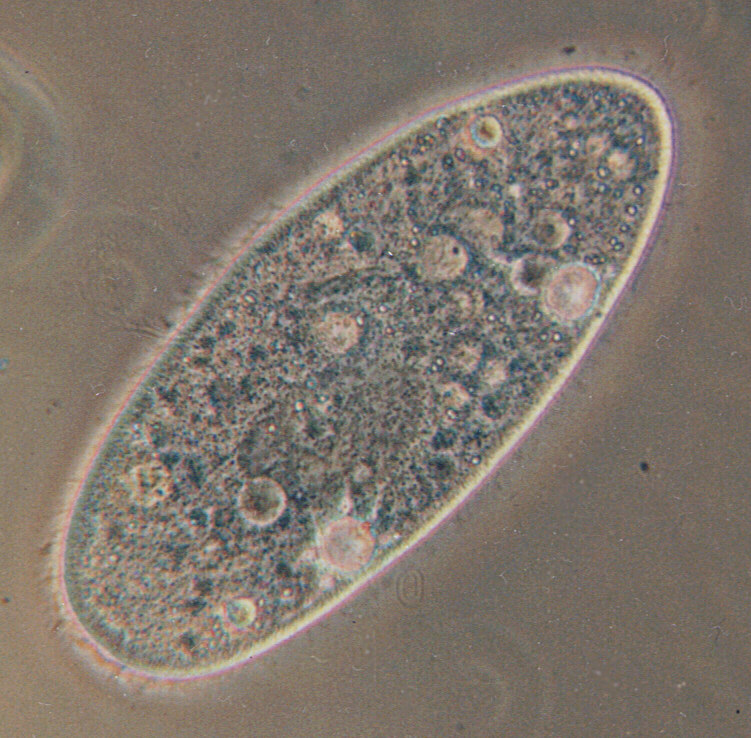
\includegraphics[width=0.97\textwidth]{Figures/Paramecium.jpg}
%     \caption{Picture of a paramecium. \cite{wikipedia}}
%     \label{fig:paramecium}
%     \end{figure}
% \end{minipage}

% \noindent
% \begin{minipage}{0.49\textwidth}

% \vspace{1.2em}

% \subsection{Galvanotaxis}
% There are four reactions possible when an electric field is applied to paramecium:

% \begin{itemize}
%     \item No response
%     \item Ciliary reversal
%     \item Cell's contraction
%     \item Cell's death
% \end{itemize}

% Figure \textbf{\ref{fig:cell_response}} shows how cells react to the electric field as a function of the pulse strength and duration.

% \end{minipage}
% \hfill
% \begin{minipage}{0.49\textwidth}
%     \begin{figure}[H]
%     \centering 
%     \captionsetup{width=0.9\linewidth, justification=centering}
%     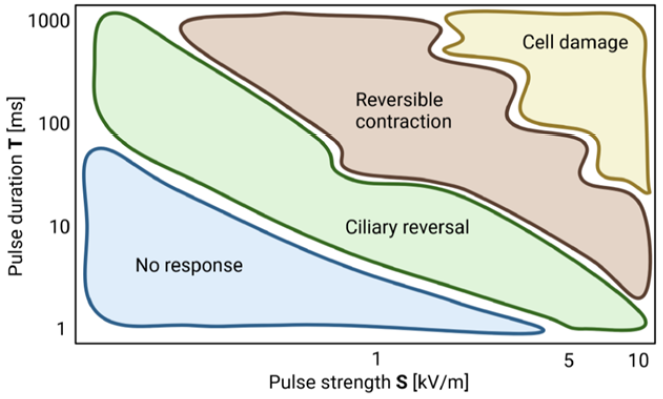
\includegraphics[width=1\textwidth]{Figures/Cell_response.png}
%     \caption{Paramecium's response as a function of the pulse strength and duration. \cite{Notice}}
%     \label{fig:cell_response}
%     \end{figure}
% \end{minipage}



% \subsection{Ciliary reversal}

% Paramecium responds to an external electric field by reversing the direction of its ciliary beating, a phenomenon known as ciliary reversal. Under normal conditions, the cilia beat in a coordinated pattern from front to back, propelling the organism forward. However, when the anterior end of the cell is exposed to a cathodal electric field, the membrane depolarizes, causing voltage-gated calcium channels to open and \ce{Ca^2+} ions to enter the cell. This calcium influx triggers a reversal in the ciliary beat direction, making the Paramecium swim backward. When an electric field is constantly applied, the ciliary reversal is such that the paramecium aligns with the E-field and swims towards the cathode. This response is part of the cell’s natural avoidance behavior, allowing it to reorient itself away from potentially harmful stimuli. The reversal is rapid and temporary, and once the membrane repolarizes, forward swimming resumes. \cite{naitoh1972}



% \subsection{Contraction, trichocysts expulsion and death}

% Paramecium exhibits a rapid contraction response when exposed to an external electric field, a phenomenon often referred to as electroshock response. When a strong enough electric stimulus is applied, the membrane becomes depolarized, causing a sudden influx of calcium ions into the cell. This triggers a rapid and temporary contraction of the cell body, often accompanied by the expulsion of trichocysts and a brief halt in movement. The response is thought to be protective, as it allows the organism to quickly react to sudden environmental changes. After the stimulus ends, the cell returns to its normal shape and resumes swimming. If the electric field is too strong or prolonged, it can lead to irreversible damage or death of the cell. \cite{naitoh1969}

% \noindent
% \begin{minipage}{0.57\textwidth}
%     Paramecium uses specialized organelles called trichocysts as a rapid defense mechanism. These elongated, capsule-like structures are embedded in the outer layer of the cell and can be explosively discharged in response to mechanical or chemical stimuli. Upon activation, each trichocyst releases a thin, filamentous thread that shoots out through the cell membrane, forming a spiky barrier around the organism. This process is believed to deter predators and is not harmful or toxic, but rather a passive defense strategy. Trichocysts can entangle or immobilize the cell itself or other cells, which can be useful in the case of predation. Trichocyst expulsion occurs rapidly (few ms) and does not require energy, relying instead on physical and ionic changes within the cell. \cite{hausmann2003}. An image of paramecium tricocysts is shown in \textbf{Figure \ref{fig:trichocysts}}.
    
% \end{minipage}
% \hfill
% \begin{minipage}{0.4\textwidth}
%     \begin{figure}[H]
%     \centering 
%     \captionsetup{width=1\linewidth, justification=centering}
%     \includegraphics[width=1\textwidth]{TP6 dying cells/Figures/trichocysts.png}
%     \caption{Paramecium trichocysts \cite{trichocysts}}
%     \label{fig:trichocysts}
%     \end{figure}
% \end{minipage}
% \noindent
% \subsection{Experimental method}

% The experiment consists in analyzing the movement of paramecium in different media and their response to an applied electric field.

% \subsubsection{Cells and media}

% Paramecium are cultured in a medium of MilliQ. This medium is used to observe the paramecium in a controlled environment. For the second medium, a solution of \ce{Ca^2+} is added to the MilliQ water. The calcium ions modify the osmotic pressure of the medium, which influences the movement of the paramecium and their response to the electric field.

% \subsubsection{Chamber}

% To observe paramecium, they are placed in a chamber. It consists of a glass slide with two thin copper foils on each side, which are used to apply the electric field. A coverslip is placed on top to create a thin volume between the slide and the coverslip. A layer scheme of the chamber is shown in figure \textbf{\ref{fig:Chamber_layer}} and a scheme of the chamber seen from the top is shown in figure \textbf{\ref{fig:Chamber_top}}. The distance between the two copper foils (width of the chamber) is 5mm. 

% \noindent
% \begin{minipage}{0.49\textwidth}
%     \begin{figure}[H]
%     \centering 
%     \captionsetup{width=0.9\linewidth, justification=centering}
%     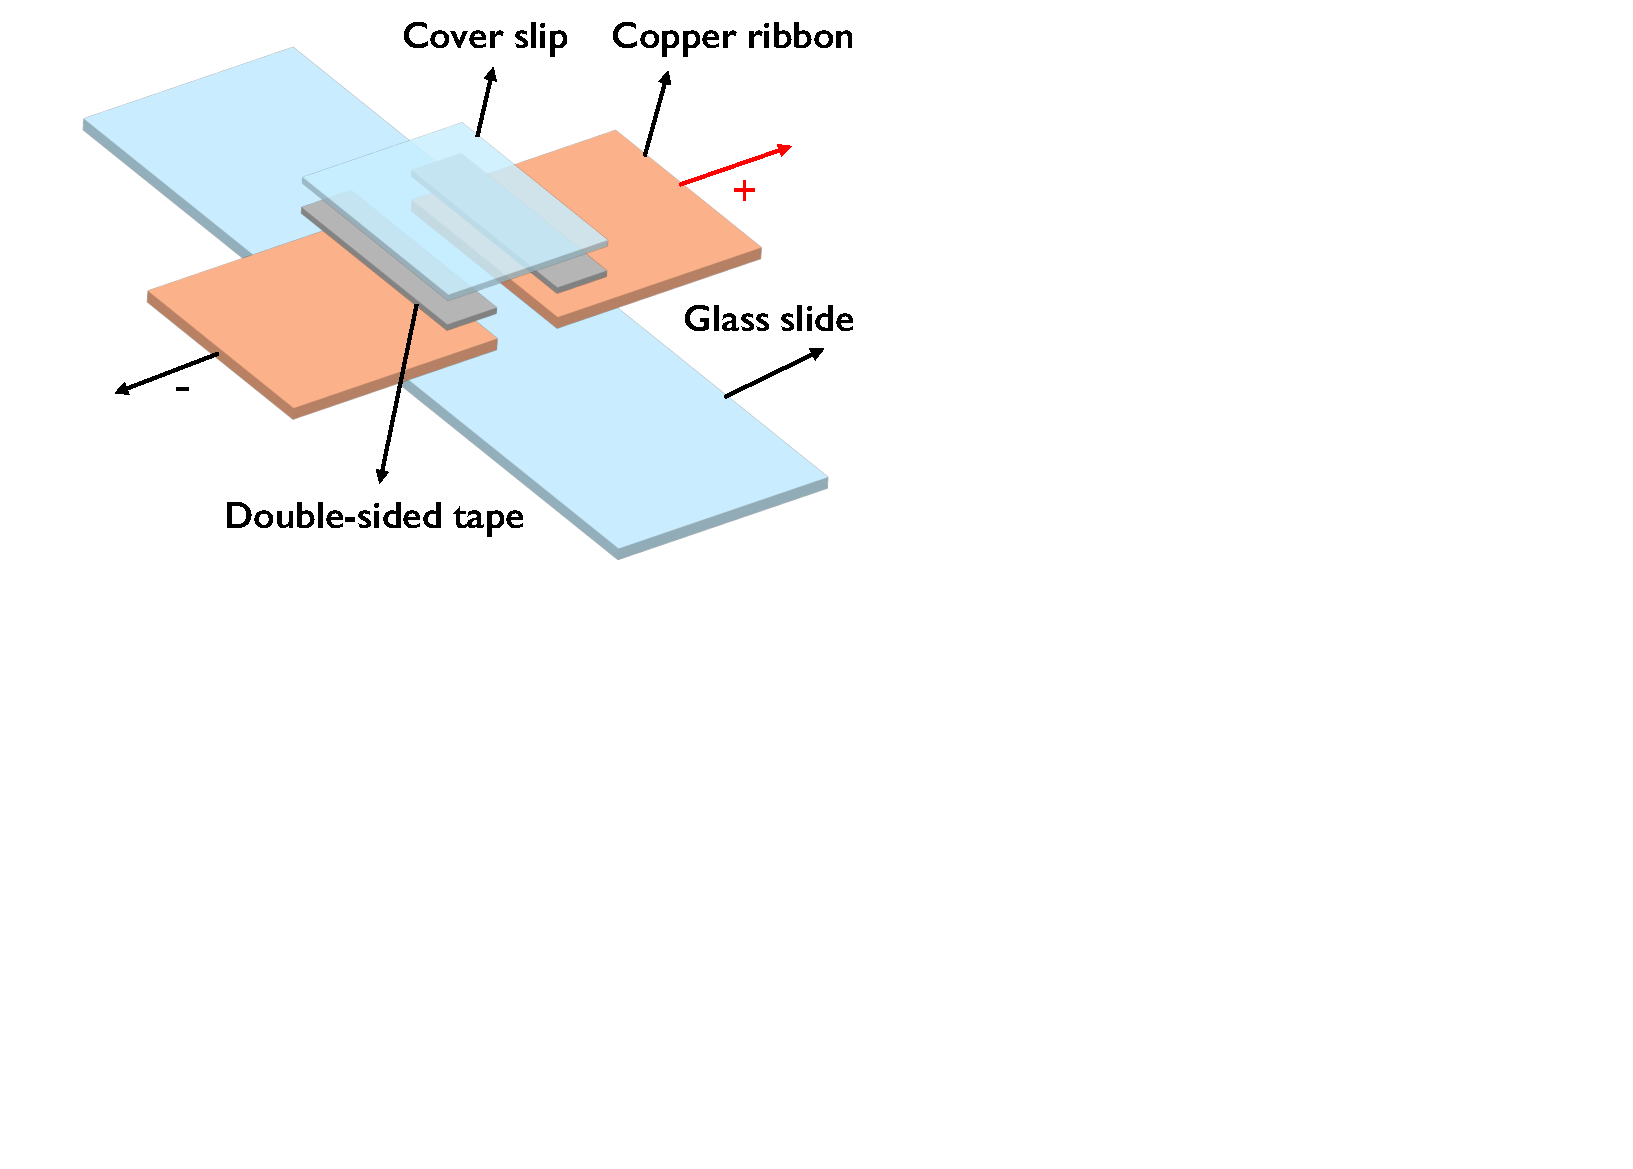
\includegraphics[width=0.9\textwidth]{Figures/Chamber_layer.pdf}
%     \caption{Layer scheme of the chamber.}
%     \label{fig:Chamber_layer}
%     \end{figure}
% \end{minipage}
% \hfill
% \begin{minipage}{0.49\textwidth}
%     \begin{figure}[H]
%     \centering 
%     \captionsetup{width=0.9\linewidth, justification=centering}
%     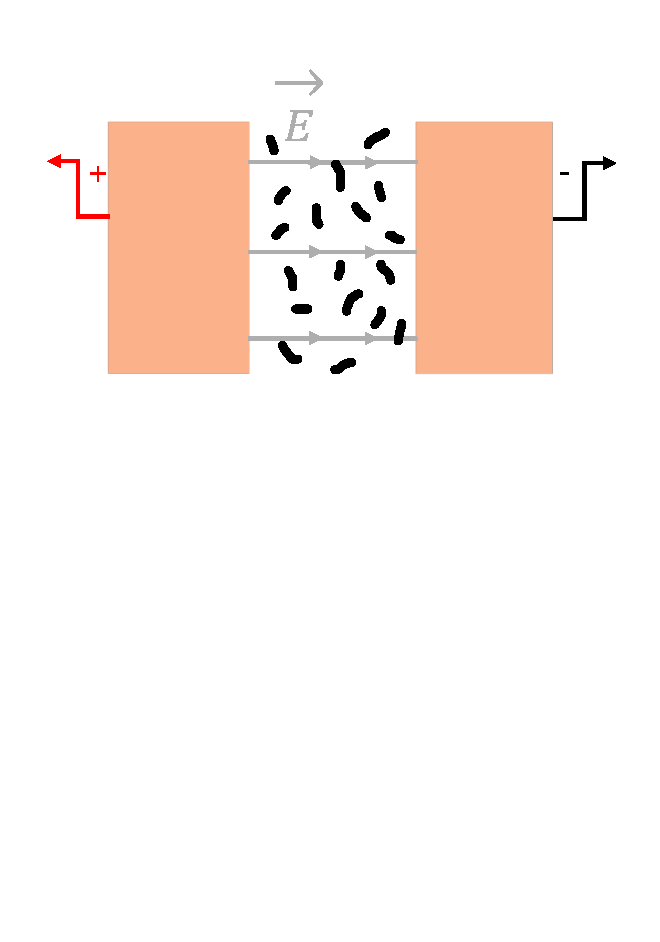
\includegraphics[width=0.9\textwidth]{Figures/Chamber_top.pdf}
%     \caption{Scheme of the chamber seen from the top.}
%     \label{fig:Chamber_top}
%     \end{figure}
% \end{minipage}

% \subsubsection{Observation and electric pulse}

% Paramecium are observed with an optical microscope. Using the microscope's program, the movement of cells can be recorded in short videos which can be exported for analysis. The electric field is applied to the chamber by connecting the copper foils to a control box. The control box allows to chose the pulse strength and duration, and is connected to a generator. A picture of the experimental setup is shown in figure \textbf{\ref{fig:setup}}.
% \begin{figure}[H]
% \centering 
% \captionsetup{width=0.9\linewidth, justification=centering}
% 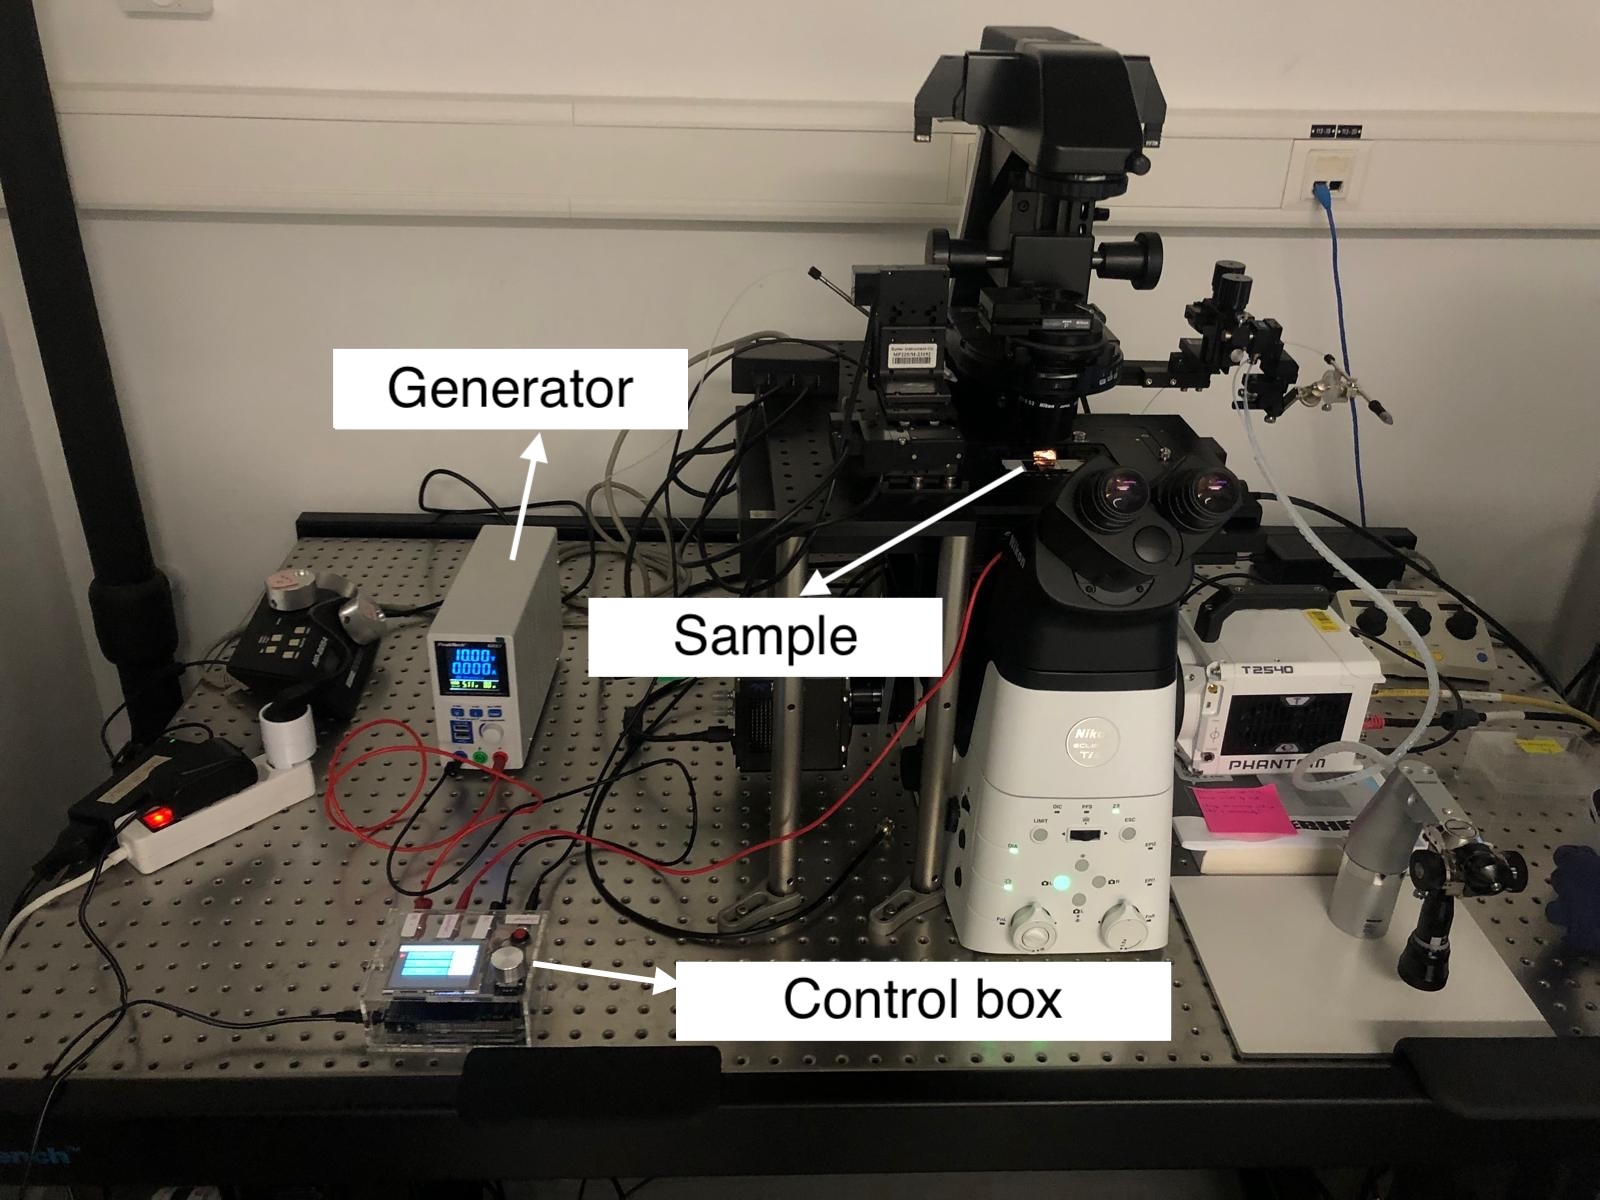
\includegraphics[width=0.7\textwidth]{Figures/gros_setup.jpeg}
% \caption{Experimental setup}
% \label{fig:setup}
% \end{figure}    
% The pulse duration is set to 1000ms and the different pulse voltages used in the experiment are 0V (no pulse), 5V, 10V, 15V and 20V, corresponding to pulse strrengths of 0V/mm, 1V/mm, 2V/mm, 3V/mm and 4V/mm respectively. The pulse is applied to the chamber while the video is being recorded. 

% \subsection{Data analysis}

% \begin{minipage}{0.49\textwidth}
% The videos were processed to extract the data using the Fiji software with the TrackMate plugin. This tool tracks cells frame by frame and records their positions as a function of time. An example of the final output from this processing is shown in \textbf{Figure~\ref{fig:trackmate}}.

% However, a technical issue during video capture with the microscope introduced lag and noise into the extracted data. To mitigate this, the cell trajectories over time were smoothed using a moving average technique. While effective in reducing noise, this method may also lead to the loss of certain details, such as brief fluctuations in speed or changes in direction.
% \end{minipage}
% \hfill
% \begin{minipage}{0.47\textwidth}
% \begin{figure}[H]
% \centering 
% \captionsetup{width=1\linewidth, justification=centering}
% 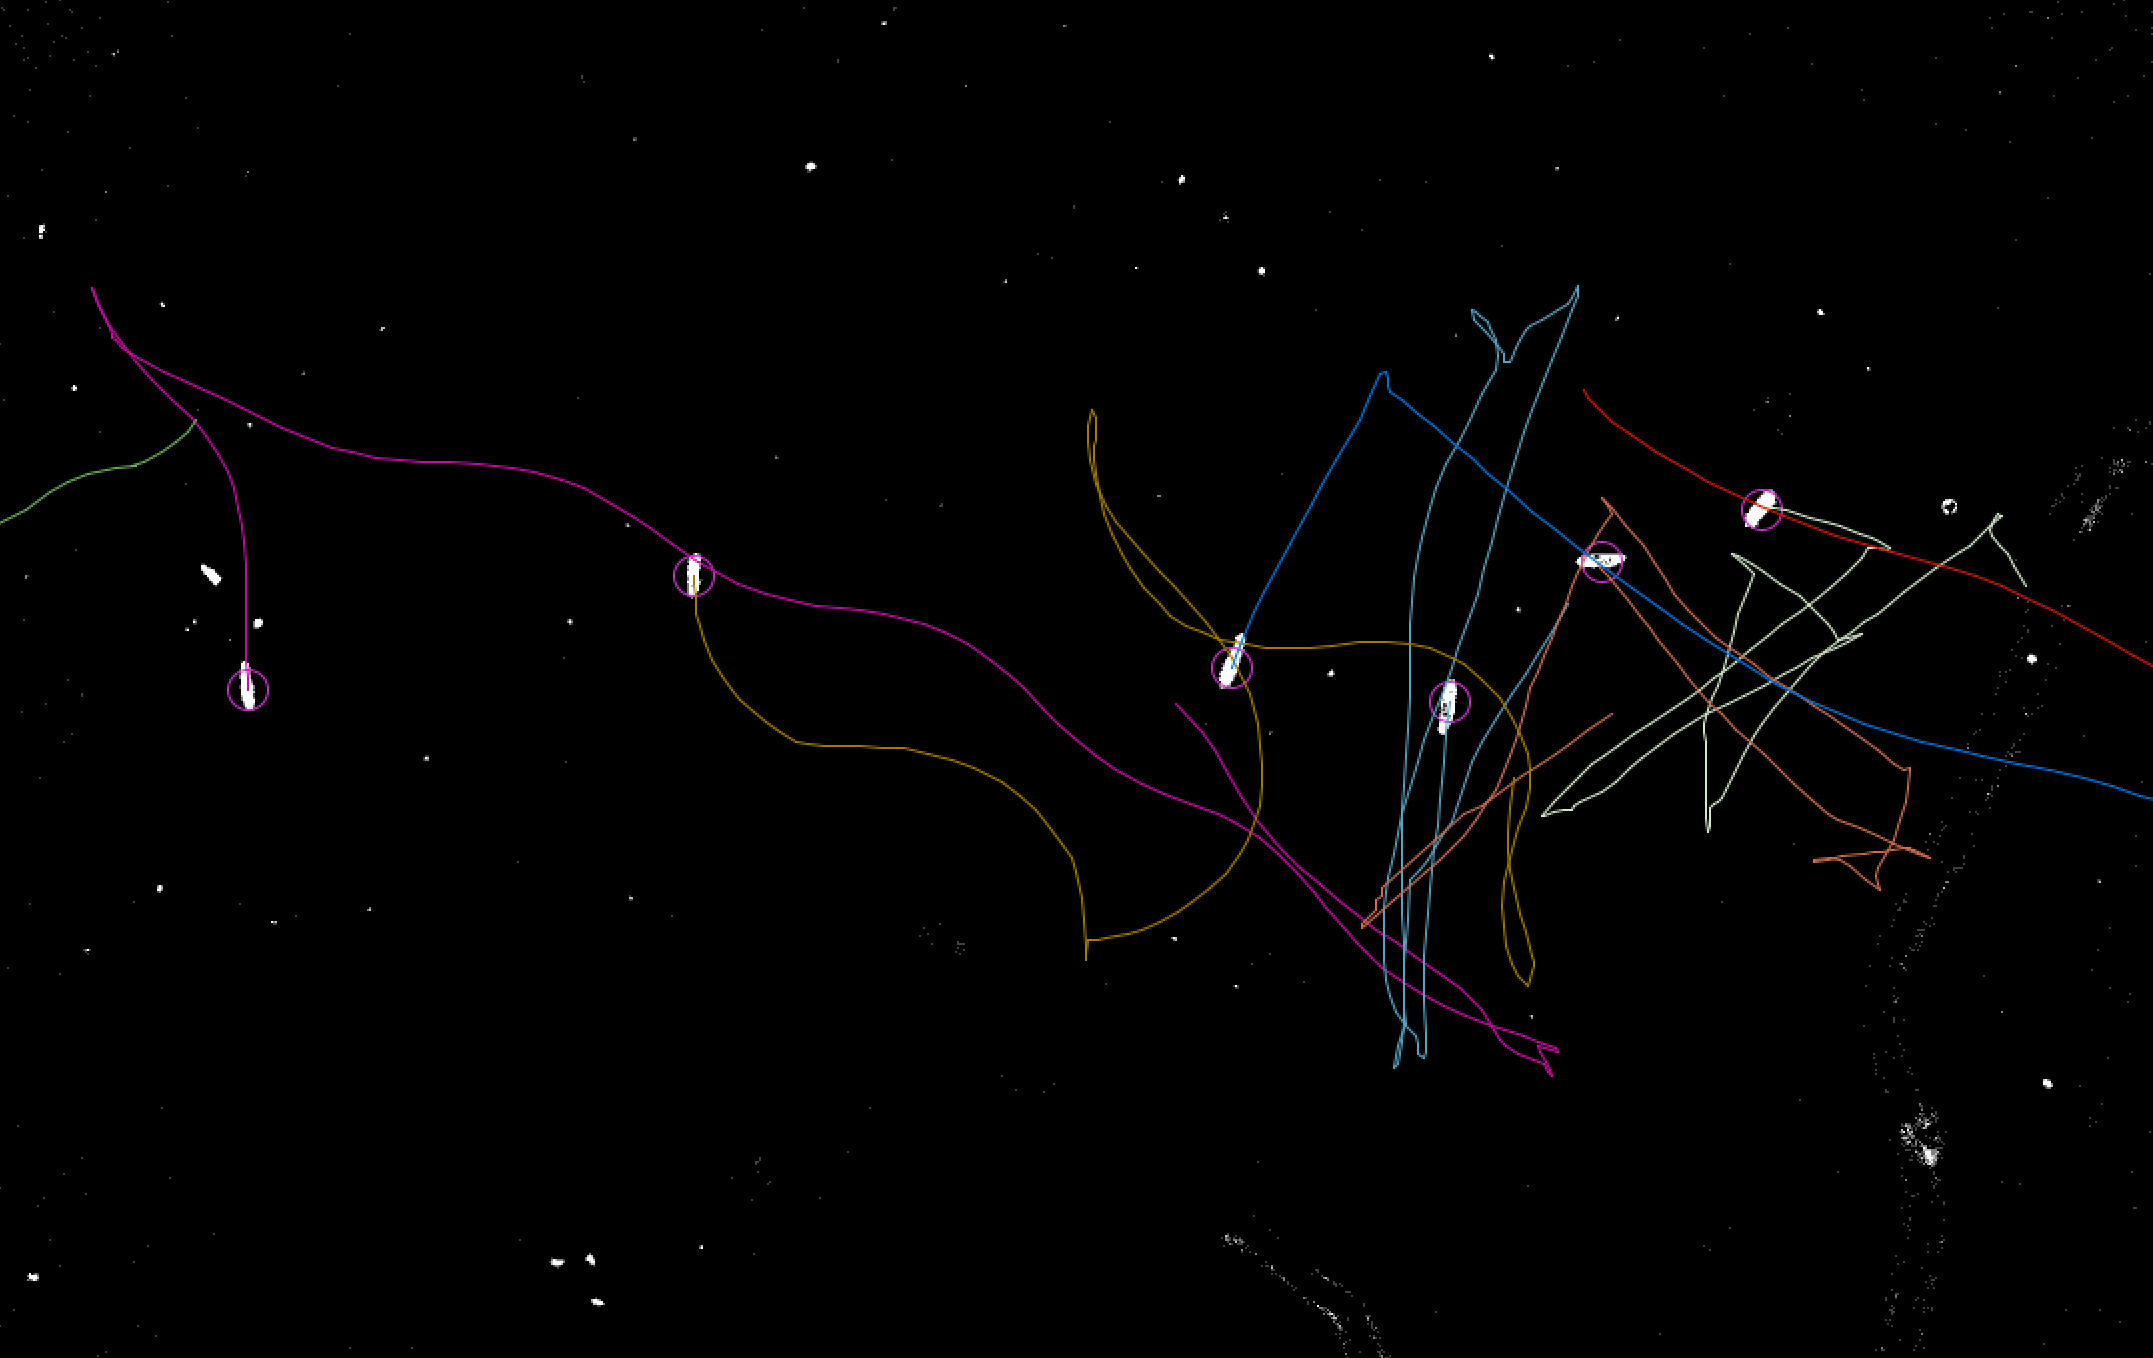
\includegraphics[width=0.9\textwidth]{Figures/Fiji.png}
% \caption{Example of a video processed with TrackMate. The white cylinders are the cells and the different trajectories are highlighted in different colors.}
% \label{fig:trackmate}
% \end{figure}
% \end{minipage}


% \section{Results and analysis}

% \subsection{Qualitative analysis}

% \paragraph{MQ vs Ca medium}
% The paramecia swim differently in the two media. In the MilliQ medium, they swim freely. When the paramecia are introduced in the \ce{Ca^2+} medium, the cells slow down and after some time, they stop moving. The cells are not dead, but in a \textbf{EXPLAIN WHAT HAPPENS} . 

% The paramecia in the \ce{Ca^2+} medium exhibit greater sensitivity to the applied electric field; specifically, their velocity norm changes more compared to those  in the MilliQ medium. This higher sensitivity will be confirmed through quantitative analysis. Furthermore, a higher number of damaged or dead paramecia are observed in the \ce{Ca^2+} medium following exposure to strong electric field pulses (15V and 20V). This is attributed to the higher ion density surrounding the paramecia in this medium, which leads to an increased ion flux into the cells and higher response

% \paragraph{Ciliary reversal}
% The first noticeable effect is that the paramecia change their direction of movement upon application of the electric pulse. This behavior is illustrated in \textbf{Figures~\ref{fig:before_pulse}} and \textbf{\ref{fig:after_pulse}}, which show the positions of the paramecia immediately before and after the application of a 20V pulse. This reversal of direction is a clear indication of ciliary reversal.

% \noindent
% \begin{minipage}{0.49\textwidth}
% \begin{figure}[H]
% \centering 
% \captionsetup{width=0.9\linewidth, justification=centering}
% 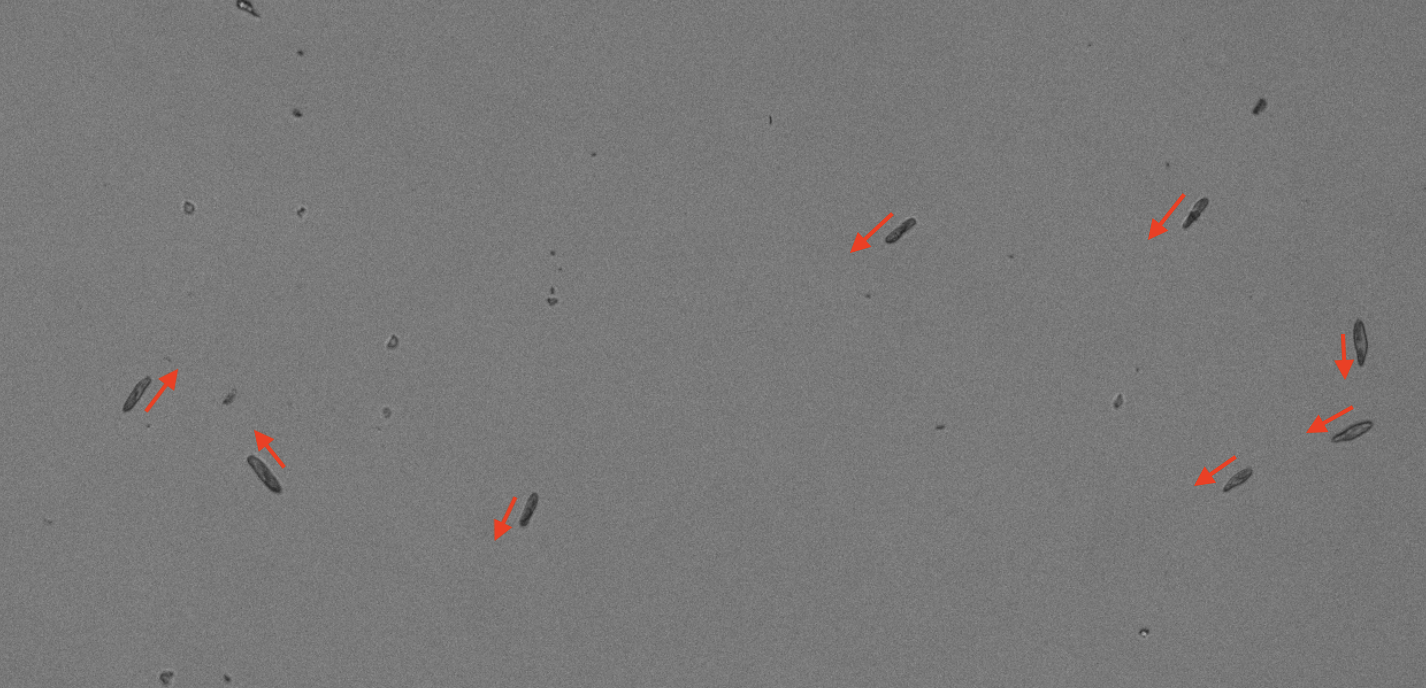
\includegraphics[width=0.9\textwidth]{Figures/before_pulse.png}
% \caption{Paramecia just before the application of the pulse.}
% \label{fig:before_pulse}
% \end{figure}
% \end{minipage}
% \hfill
% \begin{minipage}{0.49\textwidth}
% \begin{figure}[H]
% \centering 
% \captionsetup{width=0.9\linewidth, justification=centering}
% 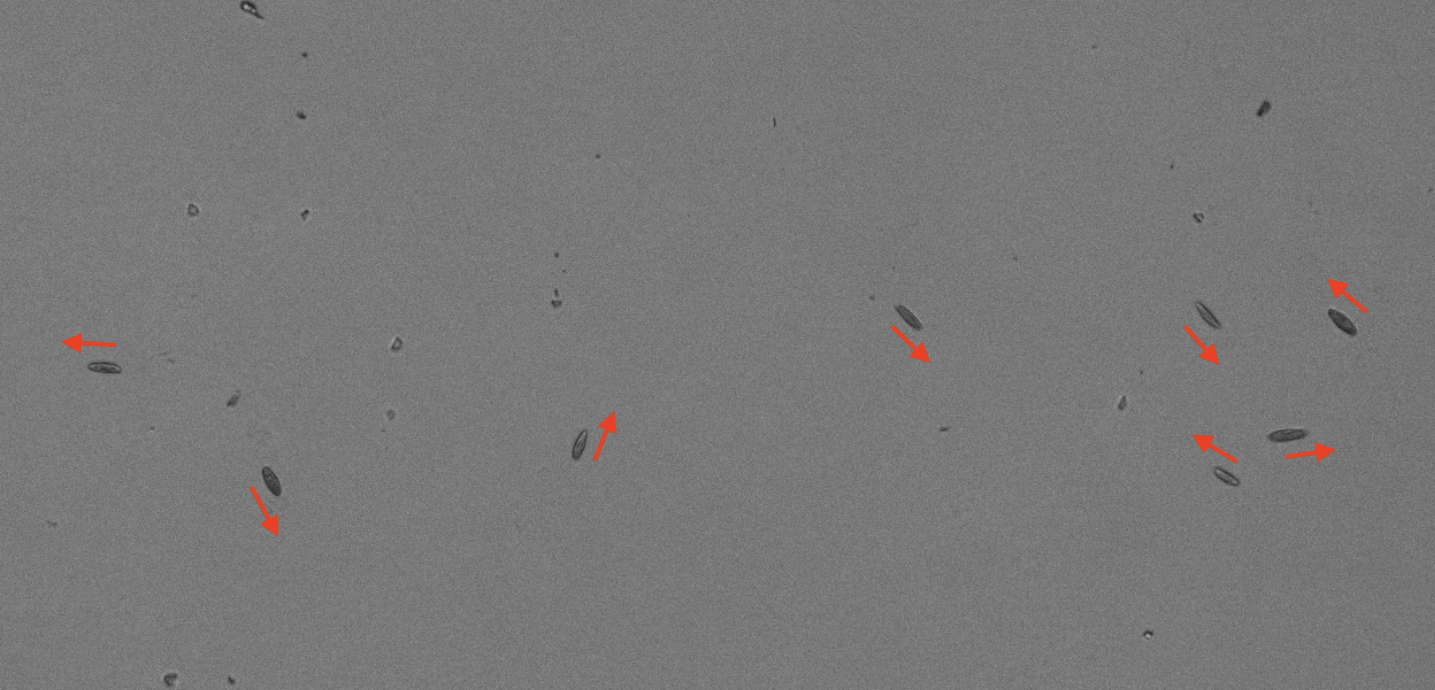
\includegraphics[width=0.9\textwidth]{Figures/after_pulse.png}
% \caption{Paramecia just after the application of the pulse.}
% \label{fig:after_pulse}
% \end{figure}
% \end{minipage}



% \paragraph{Aligning in opposition with the electric field}

% After ciliary reversal, the paramecia adjust their direction of movement to to the electric field, as long as the pulse is applied. The relatively long pulse duration used in the experiment (1000ms) enabled this behavior to be clearly observed. This alignment is more pronounced at lower voltages (5V and 10V) than at higher voltages (15V and 20V). A plausible explanation is that at higher voltages, the ciliary reversal is too strong, preventing the cells from relaxing and reorienting in time to align with the field.

% For the MilliQ medium and a pulse strength of 1V/mm, the alignement is shown in \textbf{Figure \ref{fig:aligning_before}} and \textbf{\ref{fig:aligning_during_pulse}}. The video from which these figures were extracted is available on youtube and can be seen by scanning the QR-code in \textbf{Figure \ref{fig:Paramecium_aligning}} in the appendix. 

% \noindent
% \begin{minipage}{0.49\textwidth}
% \begin{figure}[H]
% \centering 
% \captionsetup{width=0.9\linewidth, justification=centering}
% 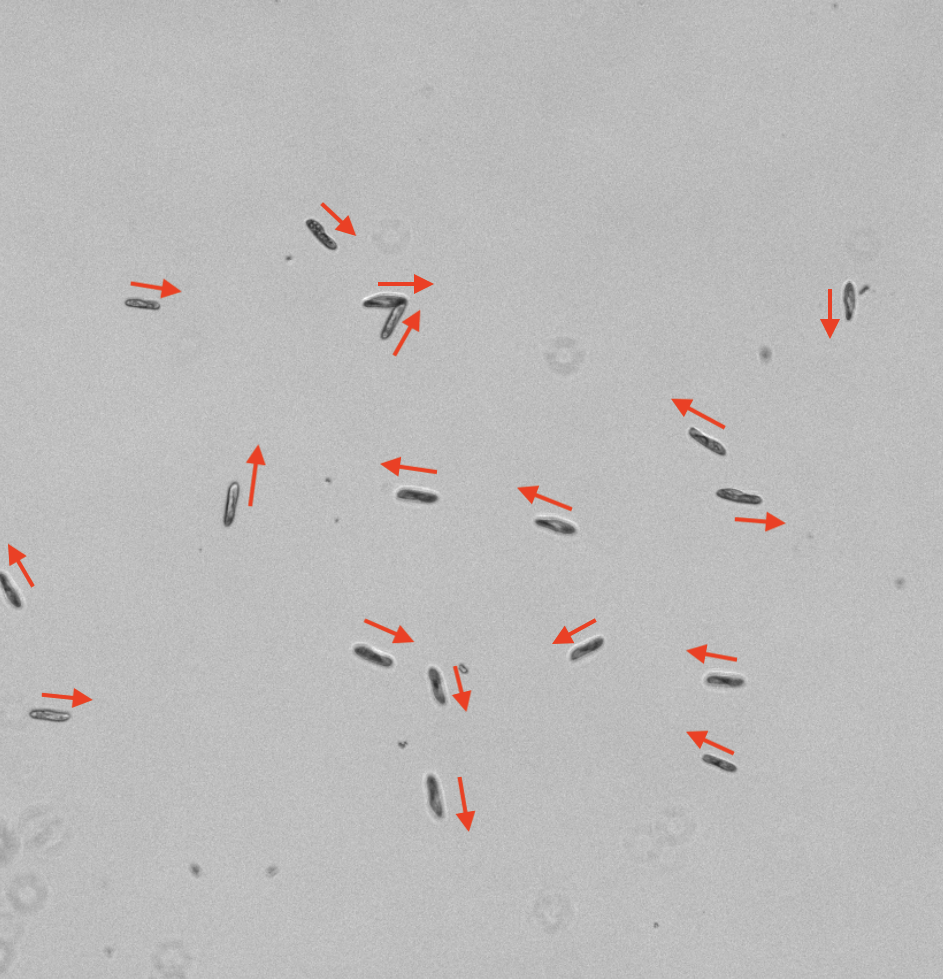
\includegraphics[width=0.8\textwidth]{Figures/aligning_before.png}
% \caption{Paramecia just before the application of the pulse, pointing in different directions.}
% \label{fig:aligning_before}
% \end{figure}
% \end{minipage}
% \hfill
% \begin{minipage}{0.49\textwidth}
% \begin{figure}[H]
% \centering 
% \captionsetup{width=0.9\linewidth, justification=centering}
% 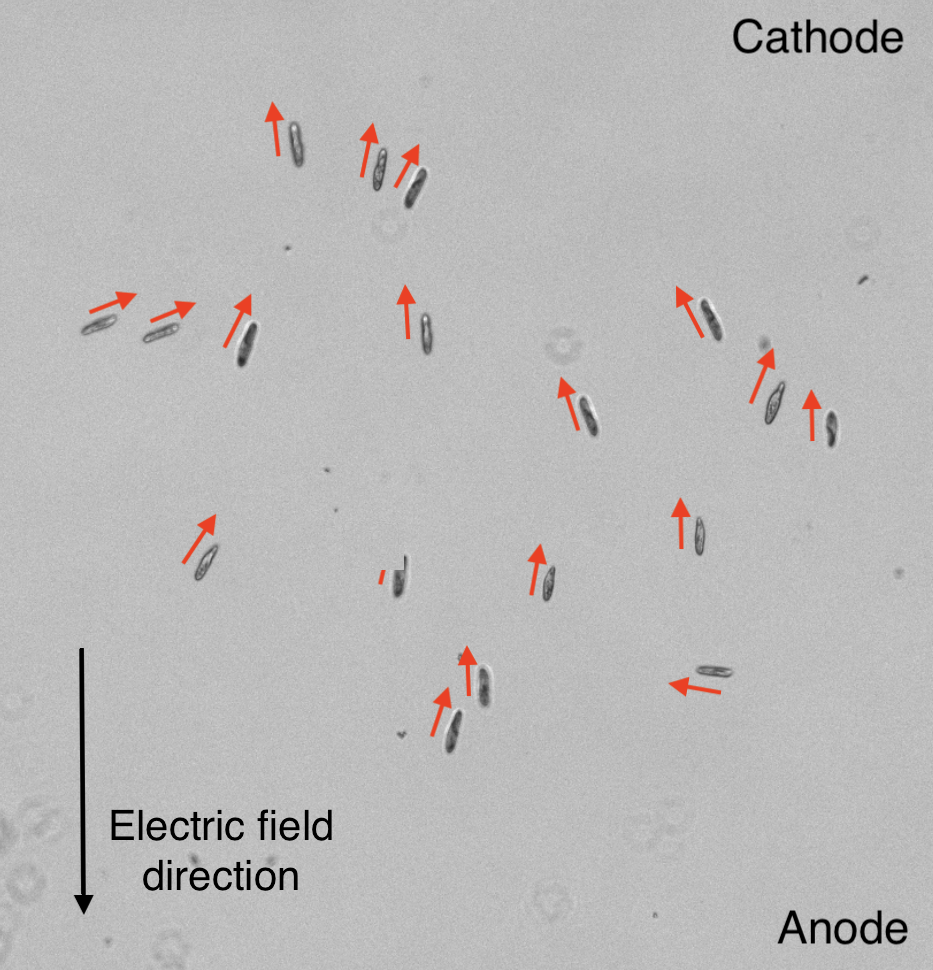
\includegraphics[width=0.8\textwidth]{Figures/aligning_during_pulse.png}
% \caption{Paramecia just after the application of the pulse, aligning in the opposite direction of the electric field.} 
% \label{fig:aligning_during_pulse}
% \end{figure}
% \end{minipage}

% \paragraph{Contraction and trichocysts expulsion}
% At high pulse strengths (15 V and 20 V), cell contraction can be observed. The contraction process for three different cells exposed to multiple consecutive 15 V pulses in MilliQ medium is illustrated in \textbf{Figure \ref{fig:Cell_in_contraction_1}}, with their state a few minutes later shown in \textbf{Figure \ref{fig:Cell_in_contraction_2}}. Additionally, a video documenting this phenomenon is available on YouTube and can be accessed by scanning the QR code in \textbf{Figure \ref{fig:Cells_contracting}} in the appendix. A fully contracted cell from the same sample, captured at higher resolution, is displayed in \textbf{Figure \ref{fig:Contracted_cell}}.

% \noindent
% \begin{minipage}{0.49\textwidth}
% \begin{figure}[H]
% \centering 
% \captionsetup{width=0.9\linewidth, justification=centering}
% 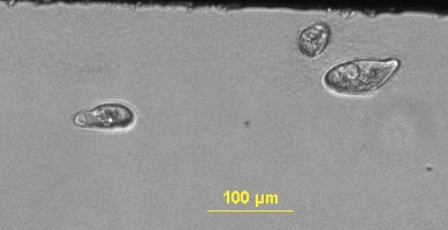
\includegraphics[width=0.9\textwidth]{Figures/Cells_in_contraction_1.png}
% \caption{Paramecia in contraction.}
% \label{fig:Cell_in_contraction_1}
% \end{figure}
% \end{minipage}
% \hfill
% \begin{minipage}{0.49\textwidth}
% \begin{figure}[H]
% \centering 
% \captionsetup{width=0.9\linewidth, justification=centering}
% 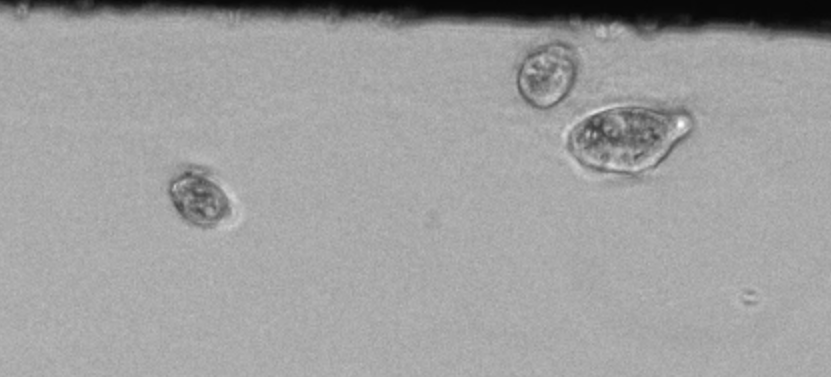
\includegraphics[width=0.9\textwidth]{Figures/Cells_in_contraction_2.png}
% \caption{Paramecia in contraction after a couple of minutes.}
% \label{fig:Cell_in_contraction_2}
% \end{figure}
% \end{minipage}
% In the video, the movement of the cytoskeleton in one paramecium can be directly observed. The cilia of this cell are beating rapidly but in a disorganized manner, indicating cellular damage. Because the cilia cannot beat properly, the cell is unable to swim. As described in the theory section, both contraction and ciliary disorganization are responses to the applied electric field.

% Within the same sample, some paramecia expelled their trichocysts and became stationary or spinning around their longitudinal axis. An example of a paramecium expelling trichocysts while spinning is shown in \textbf{Figure \ref{fig:Trichocysts_expulsion}}. A video capturing this process in two other paramecia is available on YouTube and can be accessed by scanning the QR code in \textbf{Figure \ref{fig:Swimming_Damaged_Paramecium}} in the appendix.

% \noindent
% \begin{minipage}{0.49\textwidth}
% \begin{figure}[H]
% \centering 
% \captionsetup{width=0.9\linewidth, justification=centering}
% 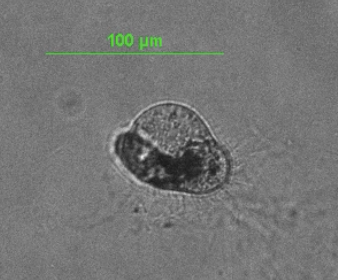
\includegraphics[width=0.9\textwidth]{Figures/Contracted_cell.png}
% \caption{Contracted paramecium}
% \label{fig:Contracted_cell}
% \end{figure}
% \end{minipage}
% \hfill
% \begin{minipage}{0.49\textwidth}
% \begin{figure}[H]
% \centering 
% \captionsetup{width=0.9\linewidth, justification=centering}
% 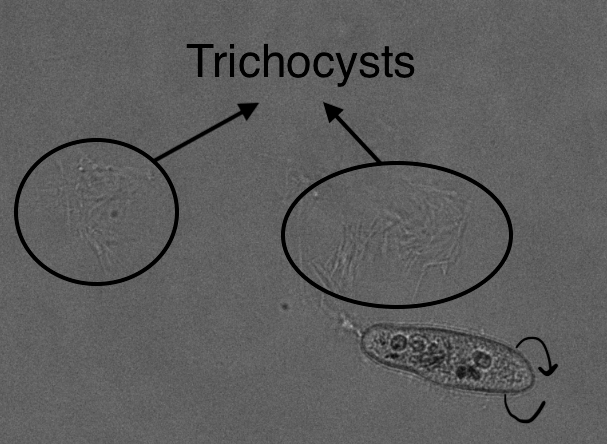
\includegraphics[width=0.9\textwidth]{Figures/Trichocysts_expulsion.png}
% \caption{Paramecium expelling trichocysts while spinning along its longitudinal axis.}
% \label{fig:Trichocysts_expulsion}
% \end{figure}
% \end{minipage}

% Trichocyst expulsion reflects an excessive ionic flux across the cell membrane, to which the paramecium reacts by expelling these organelles (see theory). In these cases, the ionic flux caused important damages to the cells, making them unable to swim properly. Some cells may also me stuck in their own trichocysts, this is the case of one of the paramecia in the video (\textbf{Figure \ref{fig:Swimming_Damaged_Paramecium}}).


% \subsection{Quantitative analysis}

% \noindent
% \begin{minipage}{0.39\textwidth}

%     \paragraph{Trajectories of paramecium}
    
%     As explained in the theory section, paramecium typically move along one of three main types of trajectories: linear, helicoidal, or circular. Figure \textbf{\ref{fig:trajectories}} shows the different types of trajectories observed in the \ce{Ca^2+} medium without any electric stimulation. These were extracted from video recordings using the Fiji software with the TrackMate plugin. Each colored path corresponds to a different tracked cell. The presence of more circular and helicoidal motions in the Ca\textsuperscript{2+} medium suggests an effect of calcium ions on cell behavior even in the absence of electric fields.

% \end{minipage}
% \hfill
% \begin{minipage}{0.59\textwidth}
%     \begin{figure}[H]
%     \centering 
%     \captionsetup{width=0.95\linewidth, justification=centering}
%     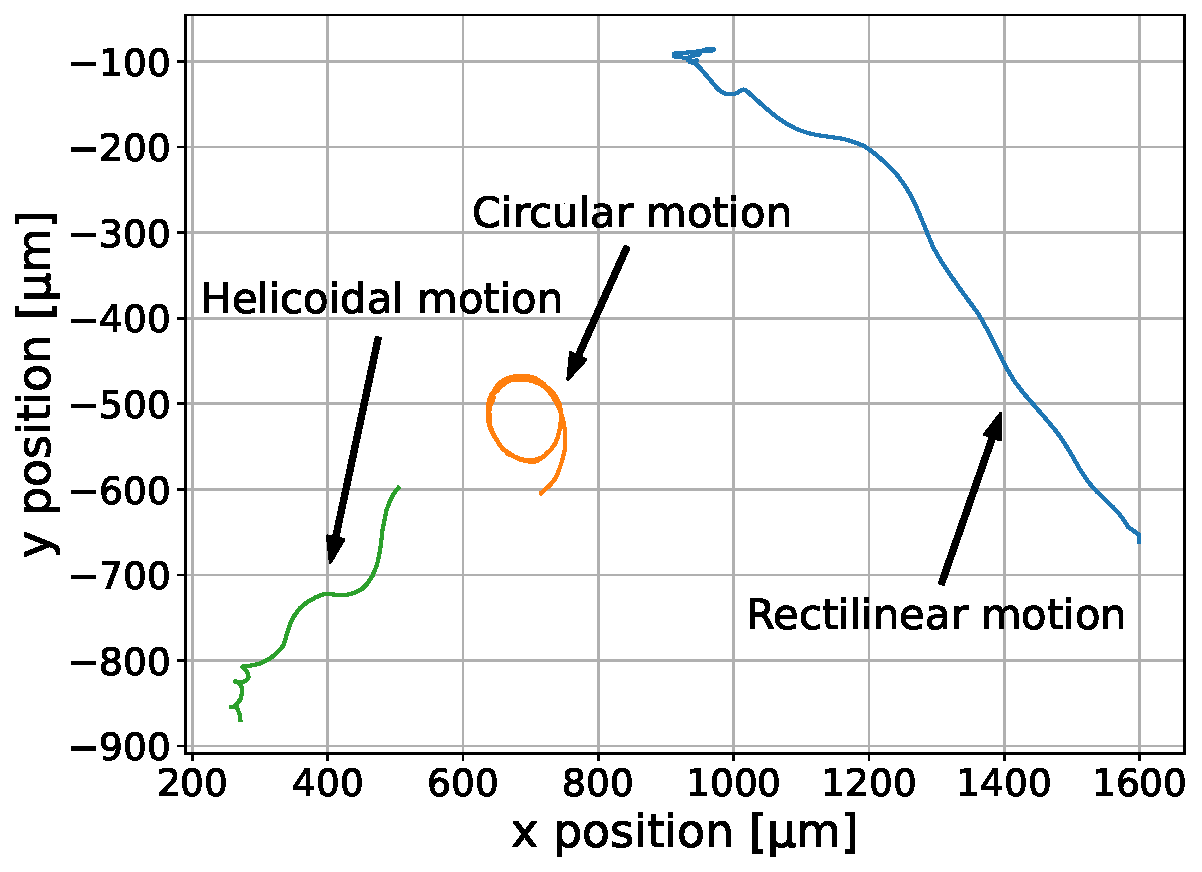
\includegraphics[width=0.9\textwidth]{Figures/2.5mM_0V_007_trajectories.pdf}
%     \caption{Different type of paramecium trajectories in the \ce{Ca^2+} medium without electric pulse.}
%     \label{fig:trajectories}
%     \end{figure}
% \end{minipage}

% \paragraph{Electric pulse response}

% Now, the response of paramecium to the electric pulse is analyzed. Velocities of paramecium are plotted as a function of time for different voltages and for the MilliQ medium in \textbf{Figure \ref{fig:velocity_all_MQ}}. The overall mean velocities (average on time and on cells) are also plotted as box-plots. The same results are plotted for the \ce{Ca^2+} medium in \textbf{Figure \ref{fig:velocity_all_Ca}}. 

% The plots in \textbf{Figure \ref{fig:velocity_all_MQ}} show that in the MilliQ medium, the paramecia remain largely unaffected by electric field pulses. There is only a slight and inconsistent stop and then increase in velocity after stimulation, which may be attributed to minor excitability of the ciliary membrane. This indicates that pure water with low conductivity does not allow for efficient electric coupling with the cells.

% In contrast, the data in \textbf{Figure \ref{fig:velocity_all_Ca}} demonstrate a significantly different behavior in the \ce{Ca^2+} enriched medium. The higher conductivity of the \ce{Ca^2+} medium enhances electric field effects across the cell membrane, allowing for stronger depolarization and consequently larger \ce{Ca^2+} influx into the cytoplasm. Cells are also slower before the pulse so the increase of velocities is much more defined.

% Furthermore, some cells exposed to higher voltage pulses (especially 15 and 20 V) displayed signs of irreversible damage, including contraction, trichocyst expulsion or death. This is consistent with the qualitative observations above. Therefore, the combination of high conductivity and strong electric field leads to overstimulation and potential cell breakdown.

% \begin{figure}[H]
%     \centering
%     \begin{subfigure}[b]{0.49\textwidth}
%         \centering
%         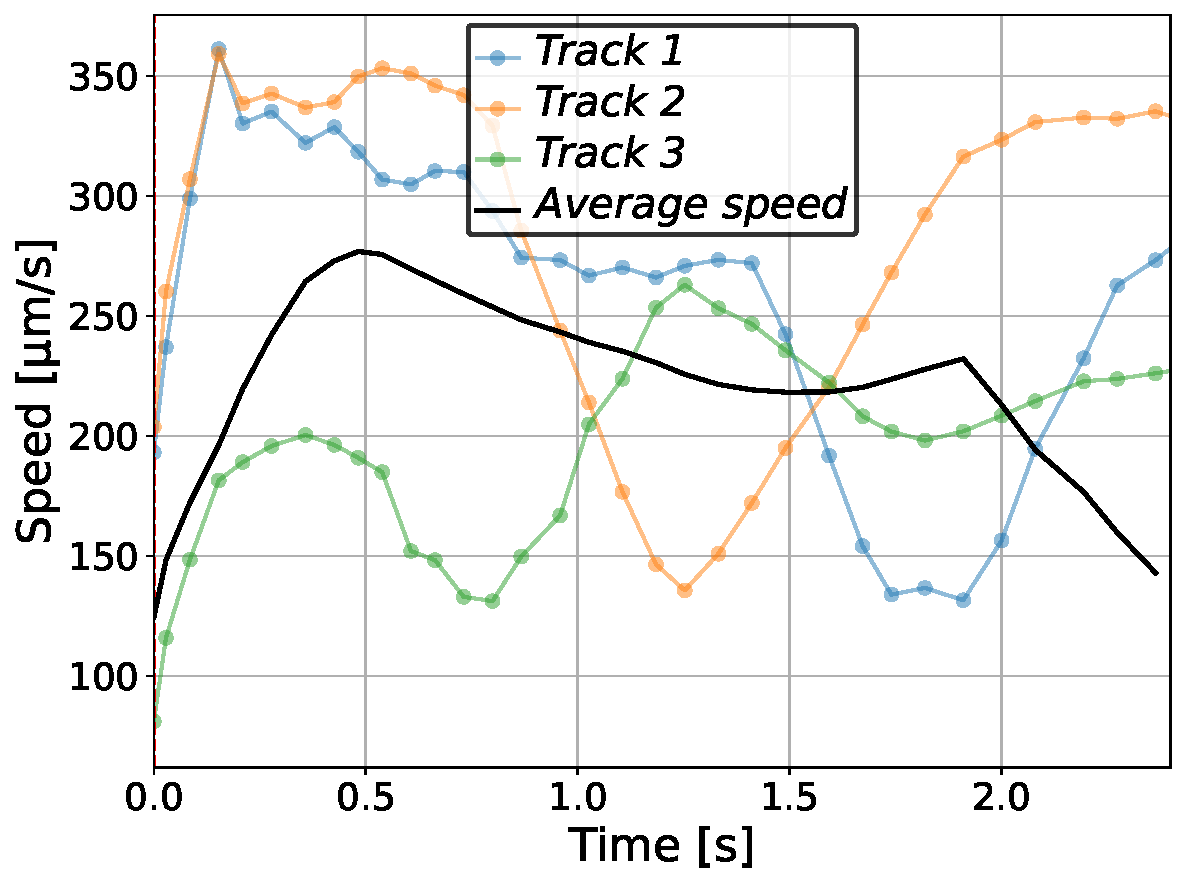
\includegraphics[width=0.95\textwidth]{Figures/MQ_0V_001_velocity_time.pdf}
%         \caption{MilliQ, 0V}
%         \label{fig:velocity_time_MQ_0V}
%     \end{subfigure}
%     \hfill
%     \begin{subfigure}[b]{0.49\textwidth}
%         \centering
%         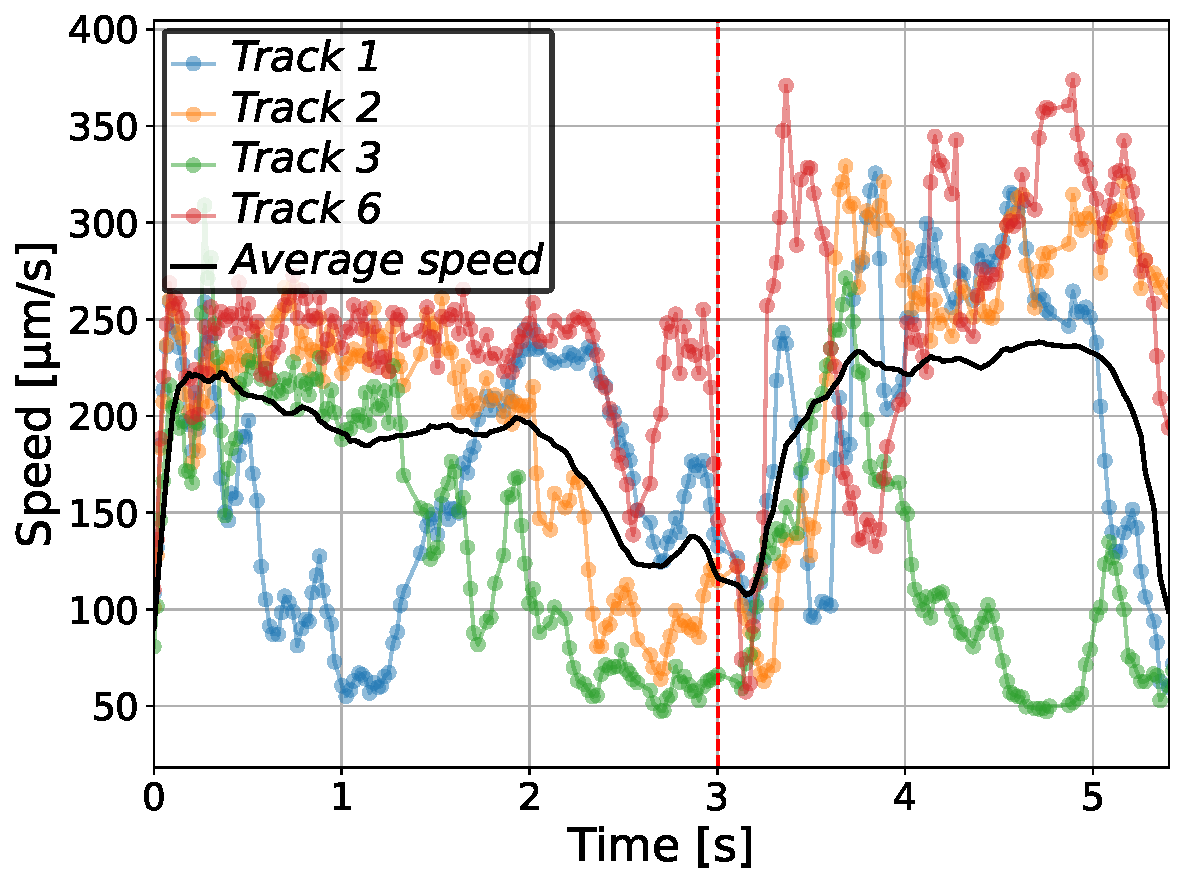
\includegraphics[width=0.95\textwidth]{Figures/MQ_5V_001_velocity_time.pdf}
%         \caption{MilliQ, 5V}
%         \label{fig:velocity_time_MQ_5V}
%     \end{subfigure}

%     \vspace{0.5em}

%     \begin{subfigure}[b]{0.49\textwidth}
%         \centering
%         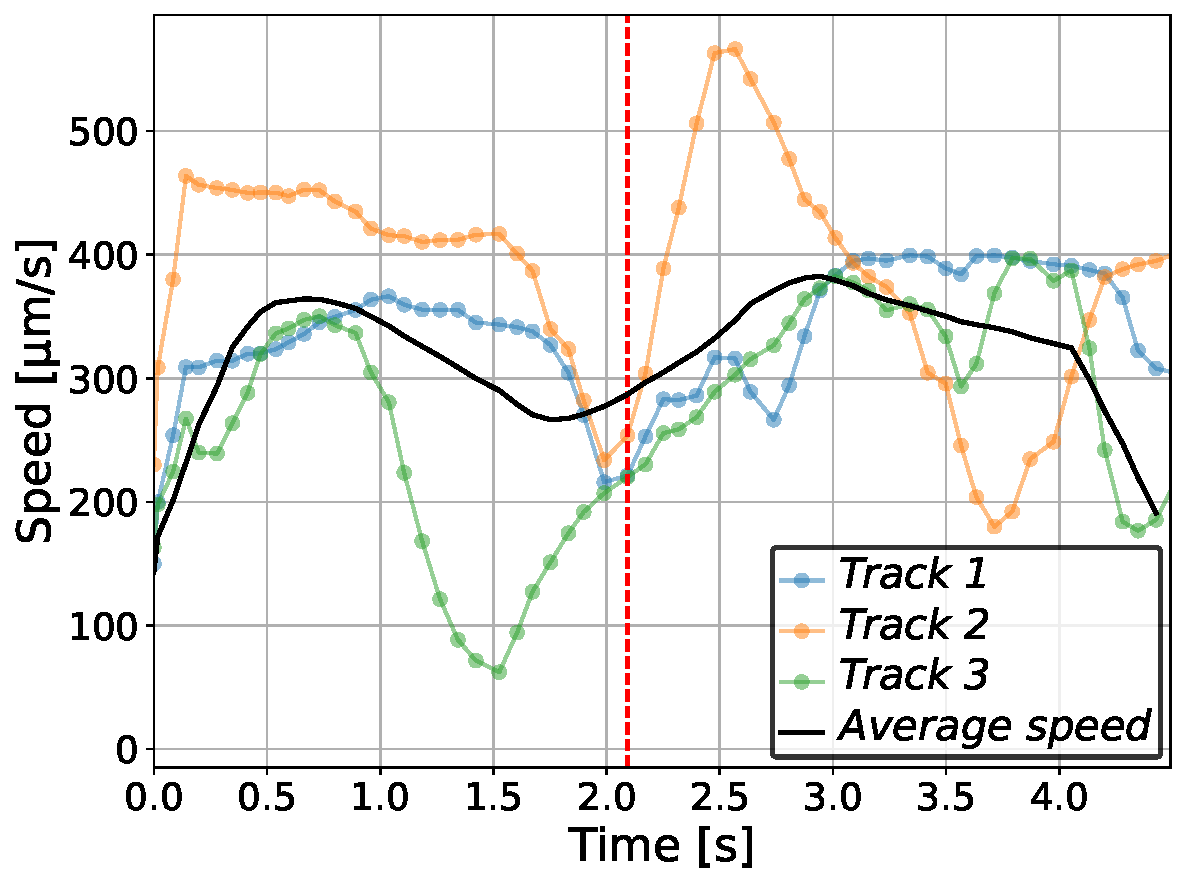
\includegraphics[width=0.95\textwidth]{Figures/MQ_10V_002_velocity_time.pdf}
%         \caption{MilliQ, 10V}
%         \label{fig:velocity_time_MQ_10V}
%     \end{subfigure}
%     \hfill
%     \begin{subfigure}[b]{0.49\textwidth}
%         \centering
%         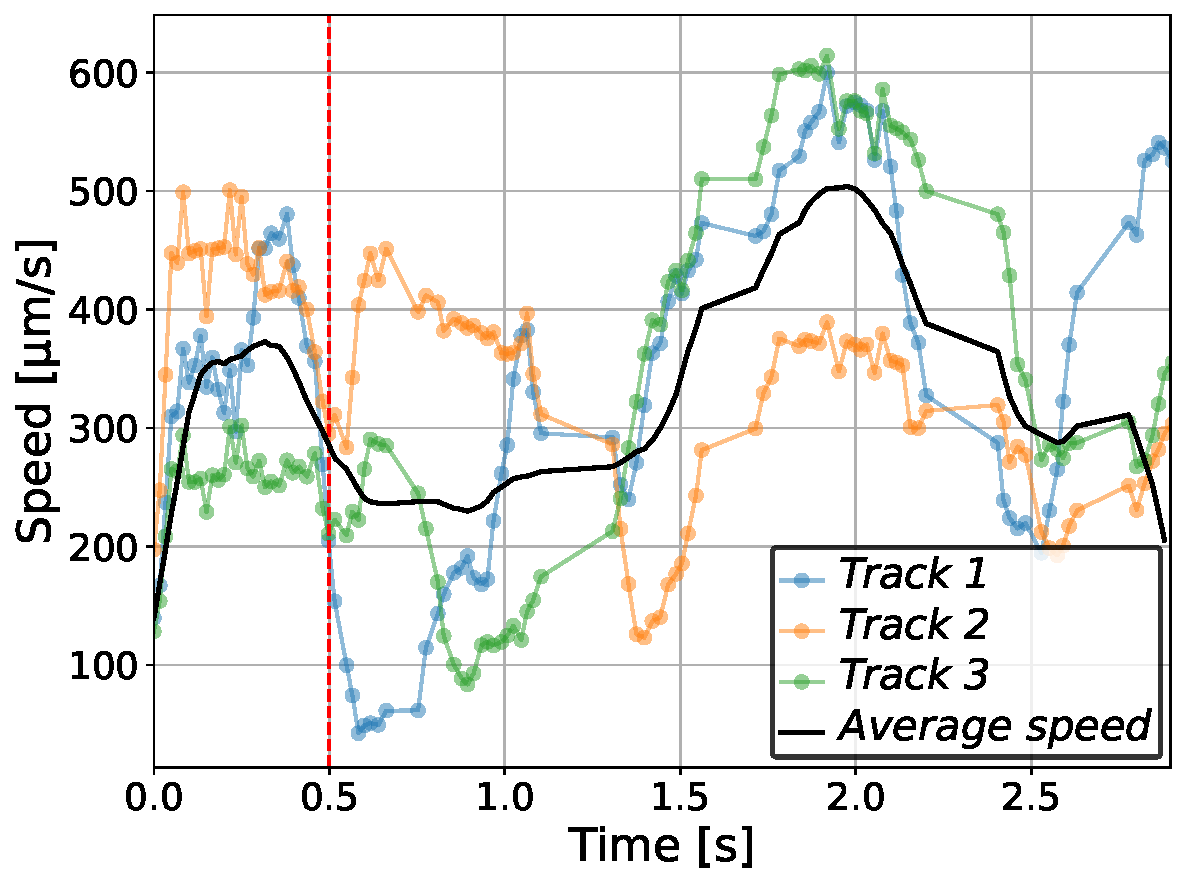
\includegraphics[width=0.95\textwidth]{Figures/MQ_15V_003_velocity_time.pdf}
%         \caption{MilliQ, 15V}
%         \label{fig:velocity_time_MQ_15V}
%     \end{subfigure}

%     \vspace{0.5em}

%     \begin{subfigure}[b]{0.49\textwidth}
%         \centering
%         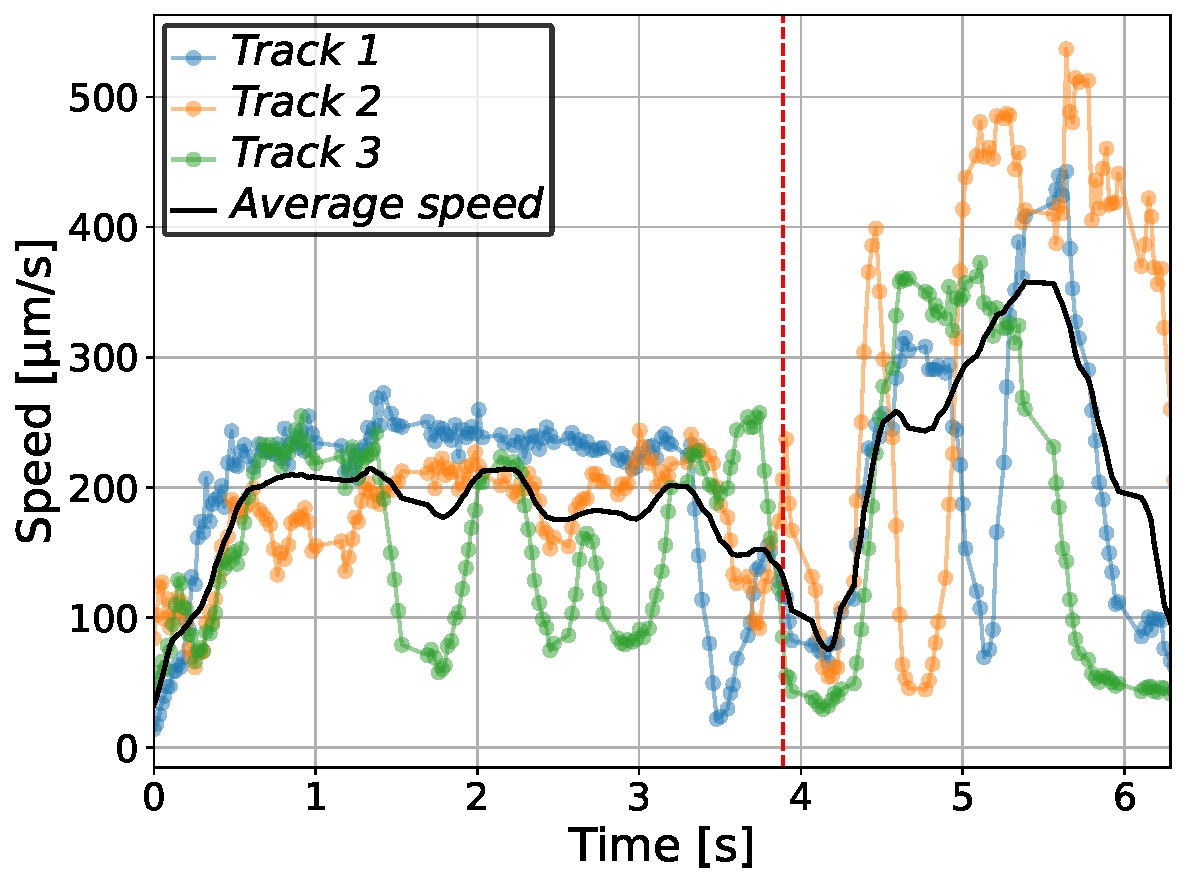
\includegraphics[width=0.95\textwidth]{Figures/MQ_20V_velocity_time.pdf}
%         \caption{MilliQ, 20V}
%         \label{fig:velocity_time_MQ_20V}
%     \end{subfigure}
%     \hfill
%     \begin{subfigure}[b]{0.49\textwidth}
%         \centering
%         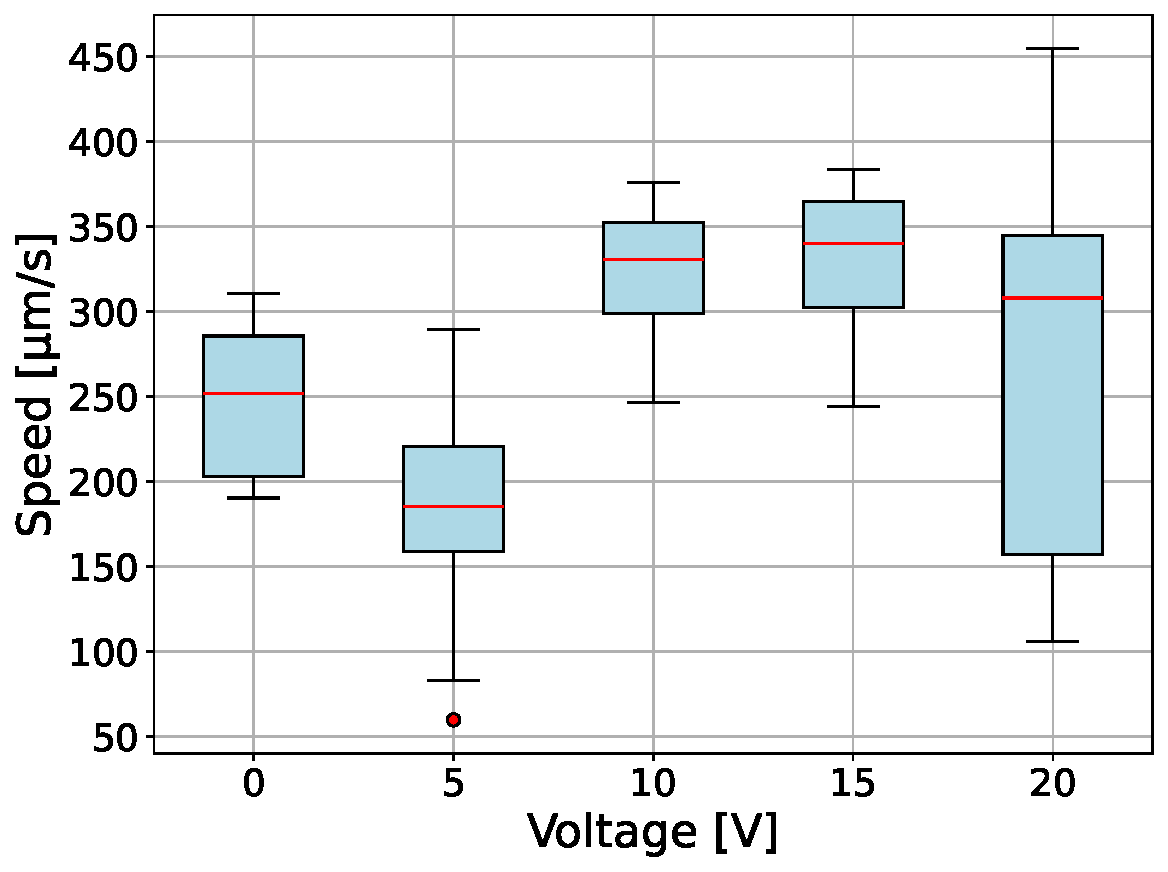
\includegraphics[width=0.95\textwidth]{Figures/MQ_velocity_vs_voltage.pdf}
%         \caption{MilliQ, Mean velocity vs voltage}
%         \label{fig:velocity_vs_voltage_MQ}
%     \end{subfigure}
%     \caption{Velocities of paramecium in the MilliQ medium as a function of time and pulse strength.}
%     \label{fig:velocity_all_MQ}
% \end{figure}


% \begin{figure}[H]
%     \centering
%     \begin{subfigure}[b]{0.49\textwidth}
%         \centering
%         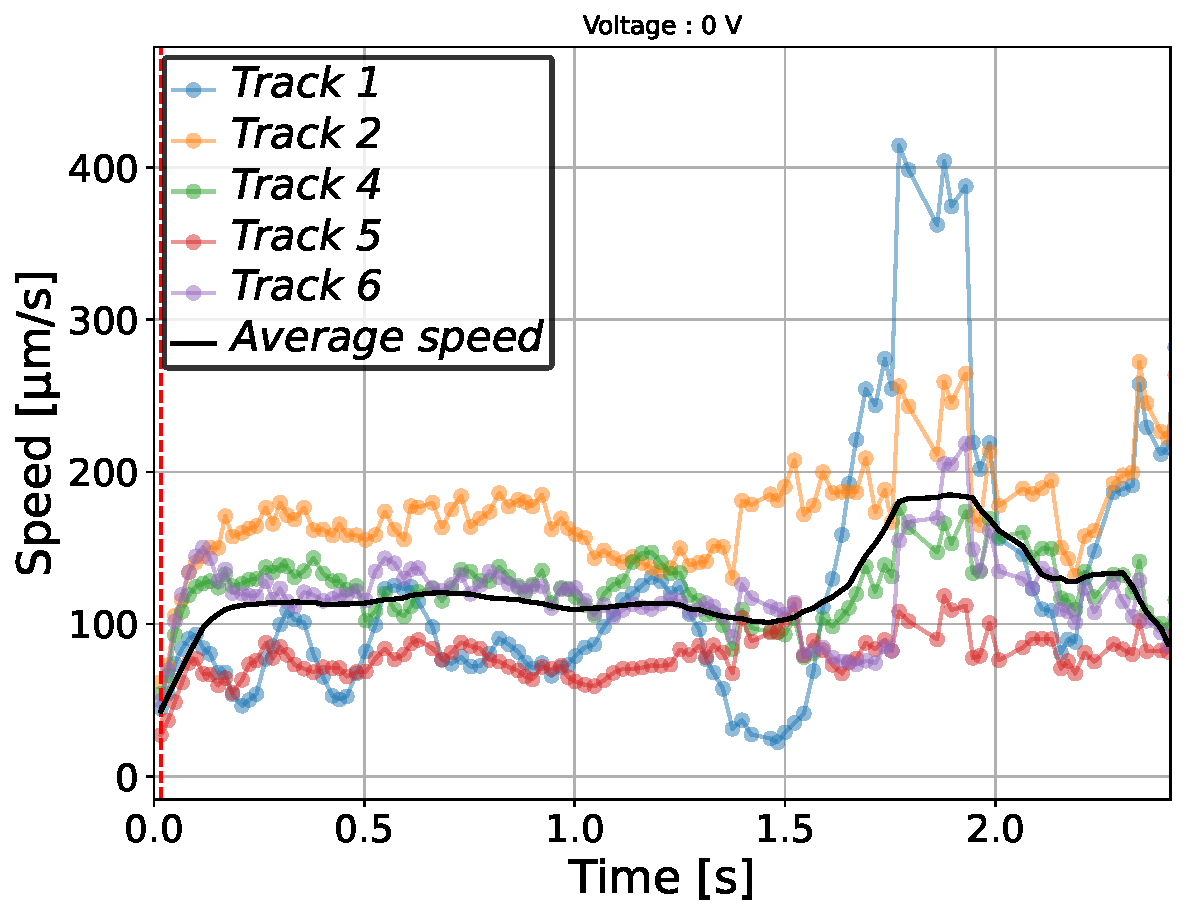
\includegraphics[width=0.95\textwidth]{Figures/2.5mM_0V_007_velocity_time.pdf}
%         \caption{\ce{Ca^2+} medium, 0V}
%         \label{fig:velocity_time_Ca_0V}
%     \end{subfigure}
%     \hfill
%     \begin{subfigure}[b]{0.49\textwidth}
%         \centering
%         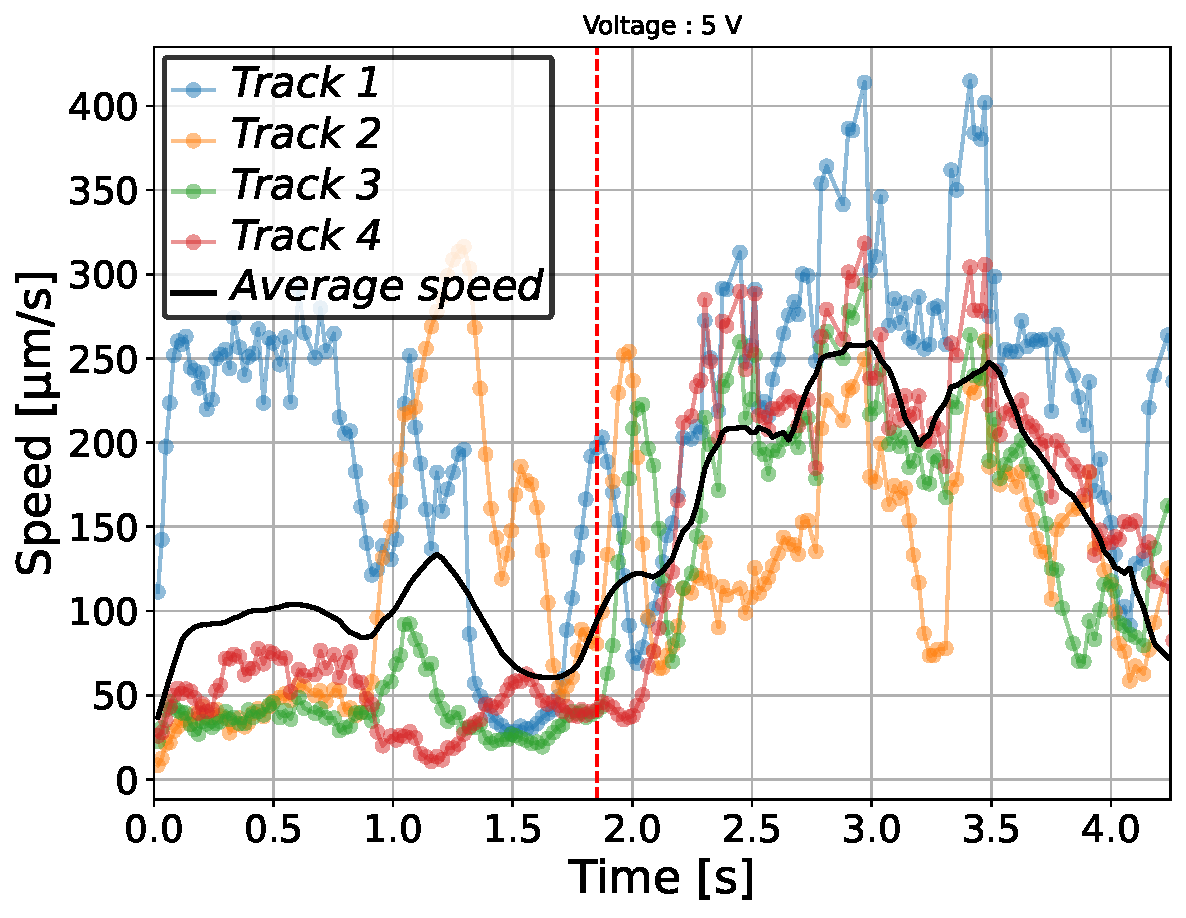
\includegraphics[width=0.95\textwidth]{Figures/2.5mM_5V_003_velocity_time.pdf}
%         \caption{\ce{Ca^2+} medium, 5V}
%         \label{fig:velocity_time_Ca_5V}
%     \end{subfigure}
%     \vspace{0.5em}
%     \begin{subfigure}[b]{0.49\textwidth}
%         \centering
%         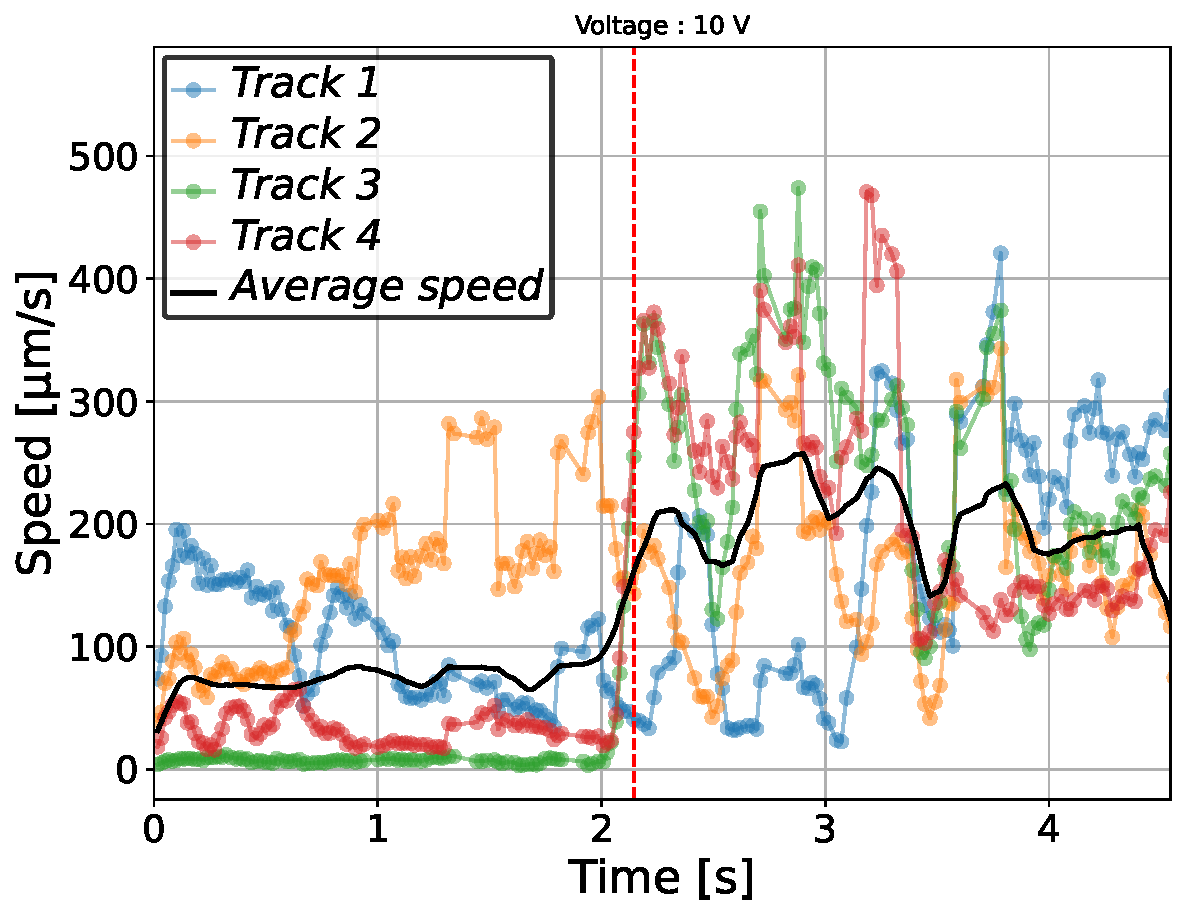
\includegraphics[width=0.95\textwidth]{Figures/2.5mM_10V_001_velocity_time.pdf}
%         \caption{\ce{Ca^2+} medium, 10V}
%         \label{fig:velocity_time_Ca_10V}
%     \end{subfigure}
%     \hfill
%     \begin{subfigure}[b]{0.49\textwidth}
%         \centering
%         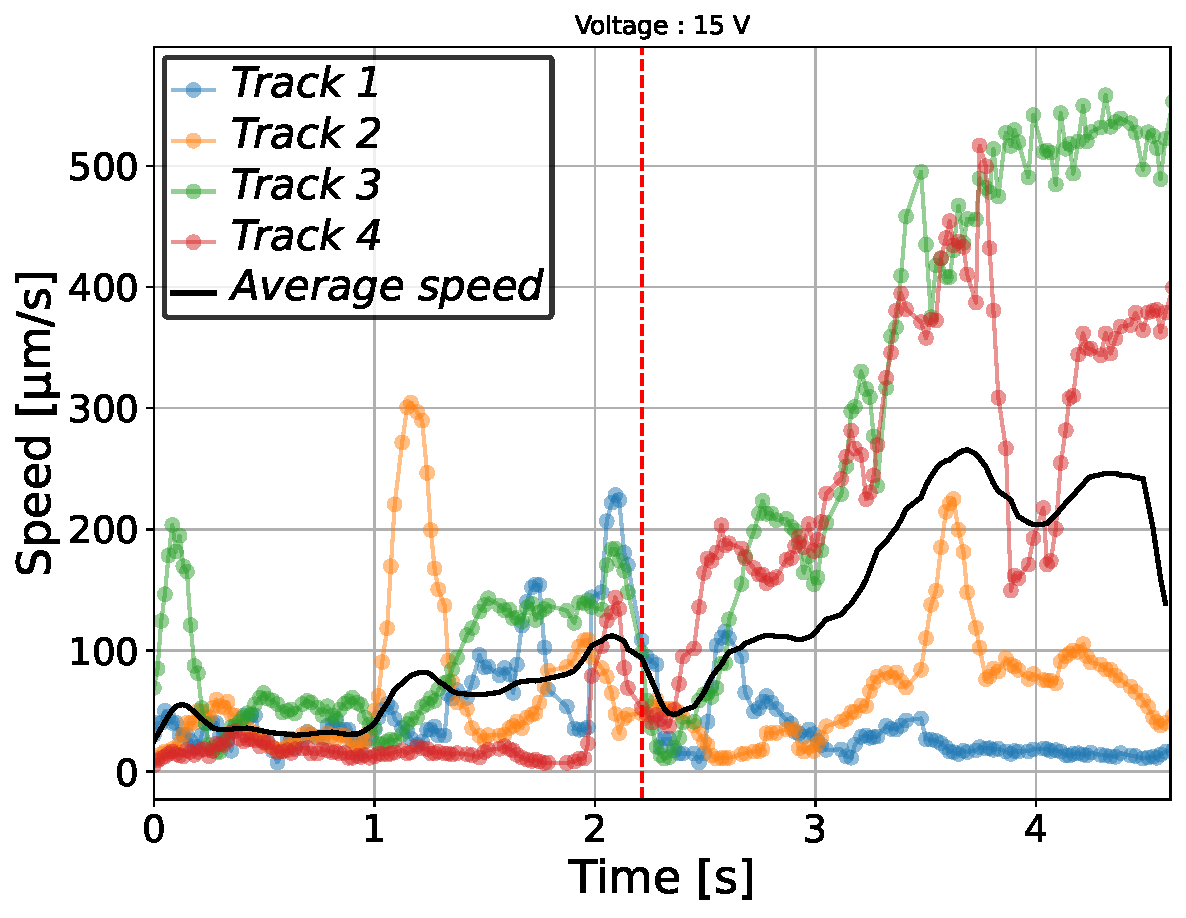
\includegraphics[width=0.95\textwidth]{Figures/2.5mM_15V_001_velocity_time.pdf}
%         \caption{\ce{Ca^2+} medium, 15V}
%         \label{fig:velocity_time_Ca_15V}
%     \end{subfigure}
%     \vspace{0.5em}
%     \begin{subfigure}[b]{0.49\textwidth}
%         \centering
%         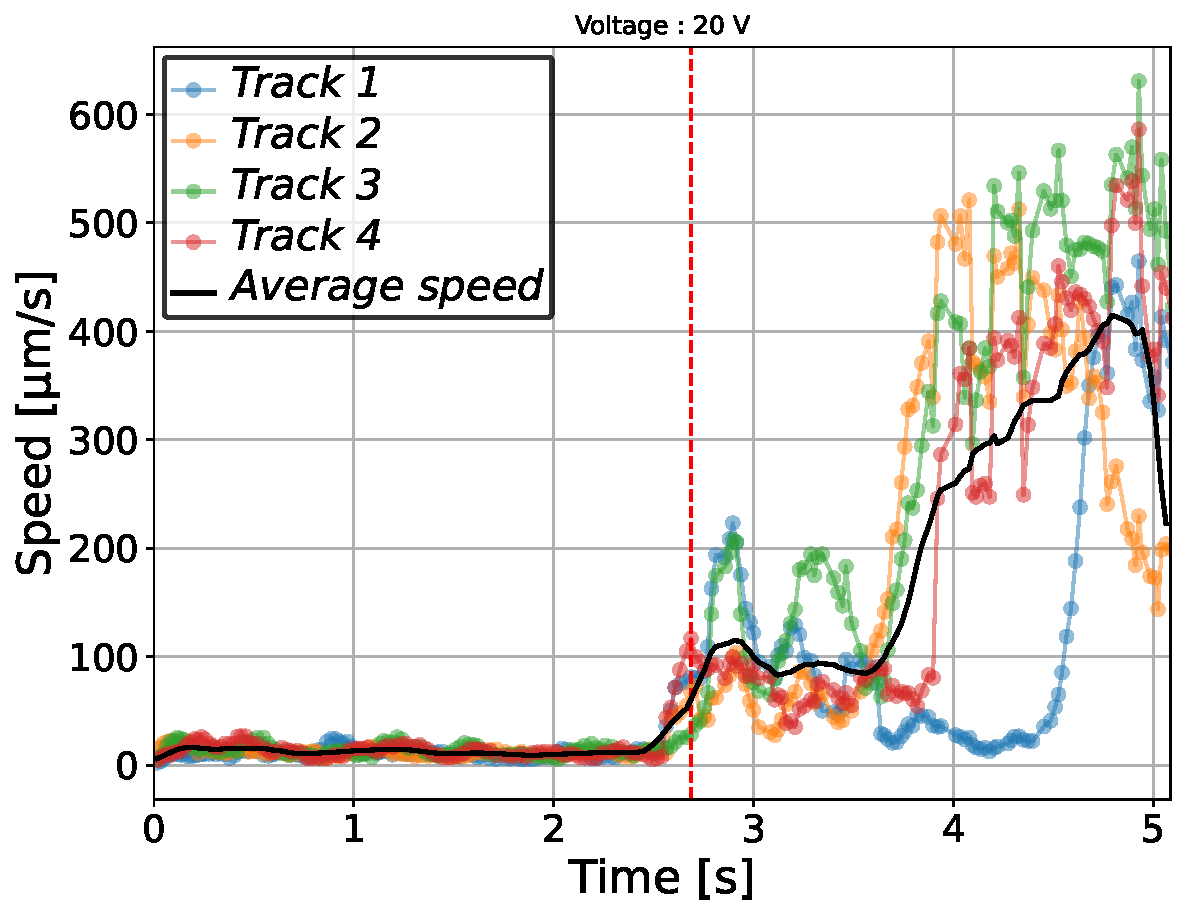
\includegraphics[width=0.95\textwidth]{Figures/2.5mM_20V_001_velocity_time.pdf}
%         \caption{\ce{Ca^2+} medium, 20V}
%         \label{fig:velocity_time_Ca_20V}
%     \end{subfigure}
%     \hfill
%     \begin{subfigure}[b]{0.49\textwidth}
%         \centering
%         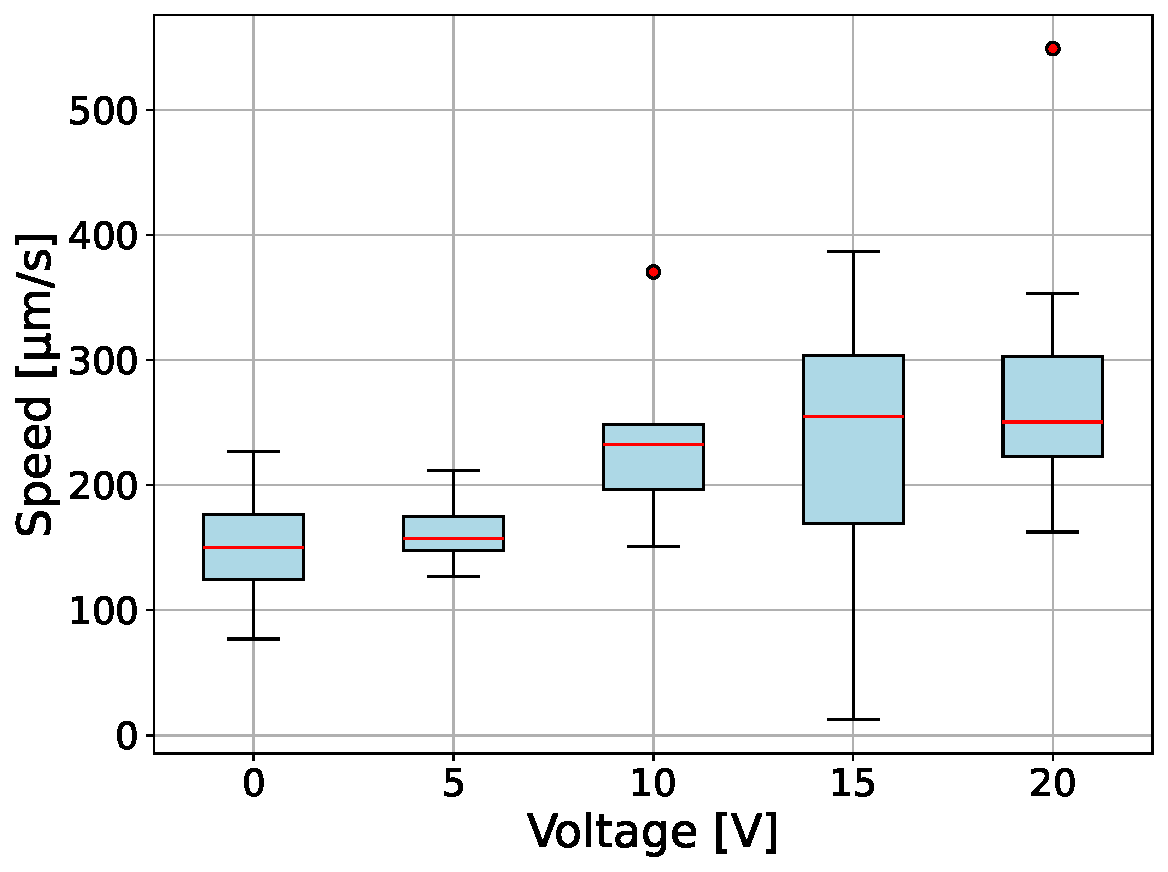
\includegraphics[width=0.95\textwidth]{Figures/2.5mM_velocity_vs_voltage.pdf}
%         \caption{Mean velocity vs voltage}
%         \label{fig:velocity_vs_voltage_Ca}
%     \end{subfigure}
%     \caption{Velocities of paramecium in the \ce{Ca^2+} medium as a function of time and pulse strength.}
%     \label{fig:velocity_all_Ca}
% \end{figure}


% Then, a statistical analysis can be made on the trajectories. One can compute the 

% \section{Conclusion}

% In this project, the response of Paramecium to electrical stimulation was studied, focusing on how different voltages and medium conductivities affect cellular behavior. Using a custom-designed observation chamber and time-resolved video microscopy, the effects of electric pulses on the motility and morphology of swimming cells were analyzed.

% Qualitative observations revealed that low-voltage pulses mainly induced ciliary reversal and directional reorientation, while higher voltages caused contraction, trichocyst expulsion, or even irreversible damage. These effects were significantly amplified in the \ce{Ca^{2+}}-enriched medium, due to its higher conductivity, which facilitates stronger membrane depolarization and \ce{Ca^{2+}} influx.

% Quantitative analysis of cell trajectories and velocities confirmed these trends. In MilliQ medium, paramecia exhibited minimal response to stimulation, while in \ce{Ca^{2+}} medium, we observed a clear increase in average speed with electric field, highlighting the role of ionic conditions in modulating electromechanical responses.

% Overall, results demonstrate that the electric field intensity and the ionic composition of the medium are key parameters in controlling the physiological responses of Paramecium. This study contributes to the understanding of rapid deformation mechanisms in protists and provides a foundation for future experiments exploring electrosensitivity in unicellular systems.



% \section{Annexes}

% \begin{minipage}{0.49\textwidth}
% \begin{figure}[H]
% \centering 
% \captionsetup{width=0.98\linewidth, justification=centering}
% 
\includegraphics[width=0.9\textwidth]{Figures/Paramecium_aligning.png}
% \caption{QR-code of the video of paramecium aligning in the opposite direction of the electric field. Link: \url{https://youtube.com/shorts/cjV4M5JLck4}}
% \label{fig:Paramecium_aligning}
% \end{figure}
% \end{minipage}
% \hfill
% \begin{minipage}{0.49\textwidth}
% \begin{figure}[H]
% \centering 
% \captionsetup{width=0.98\linewidth, justification=centering}
% 
\includegraphics[width=0.9\textwidth]{Figures/Swimming_Damaged_Paramecium.png}
% \caption{QR-code of the video of a damaged paramecium stuck in its own trichocysts and another damaged paramecium spinning along its longitudinal axis. Link: \url{https://youtube.com/shorts/yF_vT8V6dA8}}
% \label{fig:Swimming_Damaged_Paramecium}
% \end{figure}
% \end{minipage}

% \begin{figure}[H]
% \centering
% \captionsetup{width=0.9\linewidth, justification=centering}
% \includegraphics[width=0.9\textwidth]{Figures/Cells_contracting.png}
% \caption{QR-code of the video of paramecia contracting. Link: \url{https://youtube.com/shorts/NXzTY1zMing}}
% \label{fig:Cells_contracting}
% \end{figure}   


% %			Bibliographie
% \begin{thebibliography}{99}
% \bibitem{Miller1968}
% Miller, D. M., Jahn, T. L., \& Fonseca, J. R. (1968). Anodal contraction of \textit{Paramecium} protoplasm. \textit{The Journal of Protozoology}, \textbf{15}(3), 493–497. \url{https://doi.org/10.1111/j.1550-7408.1968.tb02161.x}

% \bibitem{Hausmann1976}
% Hausmann, K., \& Allen, R. D. (1976). Membrane behavior of exocytic vesicles: II. Fate of the trichocyst membranes in \textit{Paramecium} after induced trichocyst discharge. \textit{Journal of Cell Biology}, \textbf{69}(2), 313–326. \url{https://doi.org/10.1083/jcb.69.2.313}

% \bibitem{Mathijssen2019}
% Mathijssen, A. J. T. M., Culver, J., Bhamla, M. S., \& Prakash, M. (2019). Collective intercellular communication through ultra-fast hydrodynamic trigger waves. \textit{Nature}, \textbf{571}(7766), 560–564. \url{https://doi.org/10.1038/s41586-019-1387-9}

% \bibitem{wikipedia} 
% Paramécie, \textit{Paramécium}; wikipedia; \url{https://fr.wikipedia.org/wiki/Param%C3%A9cie}, visited on June 2025
% \bibitem{Notice}
% B. Noferi., Inducing ultra-fast contraction in cell shape of protists with electrical stimuli, EPFL, 2025.
% \bibitem{naitoh1972}
% Naitoh, Y., \& Kaneko, H. (1972). Reactivated triton-extracted models of \textit{Paramecium}: Modification of ciliary movement by calcium ions. \textit{Science}, \textbf{176}(4034), 523–524. \url{https://doi.org/10.1126/science.176.4034.523}
% \bibitem{naitoh1969}
% Naitoh, Y., \& Eckert, R. (1969). Ionic mechanisms controlling behavioral responses of \textit{Paramecium} to mechanical stimulation. \textit{Science}, \textbf{164}(3882), 963–965. \url{https://doi.org/10.1126/science.164.3882.963}
% \bibitem{hausmann2003}
% Hausmann, K., Hülsmann, N., \& Radek, R. (2003). \textit{Protistology}. Stuttgart: E. Schweizerbart’sche Verlagsbuchhandlung.
% \bibitem{trichocysts}
% \url{https://www.britannica.com/science/trichocyst}, visited on June 2025

% \end{thebibliography}


% \end{document}








\documentclass[a4paper, 12pt,oneside]{article}
%On peut changer "oneside" en "twoside" si on sait que le résultat sera recto-verso.
%Cela influence les marges (pas ici car elles sont identiques à droite et à gauche)

% pour l'inclusion de figures en eps,pdf,jpg,....
\usepackage{graphicx}

\graphicspath{{/workspaces/TP3/TP_Dying-cells/}}


\usepackage{float}
\usepackage{caption}
\usepackage{subcaption}
\usepackage{multirow}
\usepackage[version=4]{mhchem}


%Marges. Désactiver pour utiliser les valeurs LaTeX par défaut
%\usepackage[top=2.5cm, bottom=2cm, left=2cm, right=2cm, showframe]{geometry}
\usepackage[top=2.5cm, bottom=2cm, left=2cm, right=2cm]{geometry}

% quelques symboles mathematiques en plus
\usepackage{amsmath}

% le tout en langue francaise
%\usepackage[francais]{babel}

% on peut ecrire directement les charactères avec l'accent
\usepackage[T1]{fontenc}

% a utiliser sur Linux/Windows
%\usepackage[latin1]{inputenc}

% a utiliser avec UTF8
\usepackage[utf8]{inputenc}
%Très utiles pour les groupes mixtes mac/PC. Un fichier texte enregistré sous codage UTF-8 est lisible dans les deux environnement.
%Plus de problème de caractères accentués et spéciaux qui ne s'affichent pas

% a utiliser sur le Mac
%\usepackage[applemac]{inputenc}

% pour l'inclusion de liens dans le document (pdflatex)
\usepackage[colorlinks,bookmarks=false,linkcolor=black,urlcolor=blue, citecolor=black]{hyperref}

%Pour l'utilisation plus simple des unités et fractions
\usepackage{units}

%Pour utiliser du time new roman... Comenter pour utiliser du ComputerModern
%\usepackage{mathptmx}

%Pour du code non interprété
\usepackage{verbatim}
\usepackage{verbdef}% http://ctan.org/pkg/verbdef

%Pour changer la taille des titres de section et subsection. Ajoutez manuellement les autres styles si besoin.
\makeatletter
\renewcommand{\section}{\@startsection {section}{1}{\z@}%
             {-3.5ex \@plus -1ex \@minus -.2ex}%
             {2.3ex \@plus.2ex}%
             {\normalfont\normalsize\bfseries}}
\makeatother

\makeatletter
\renewcommand{\subsection}{\@startsection {subsection}{1}{\z@}%
             {-3.5ex \@plus -1ex \@minus -.2ex}%
             {2.3ex \@plus.2ex}%
             {\normalfont\normalsize\bfseries}}
\makeatother

%Début du document
\begin{document}


\begin{center}
\large\textbf{\sffamily Paramecium Galvanotaxis}\\%
\large\sffamily Group N$^\circ$1: Alexis Escarmelle, Nil Fajas\\%
\large\sffamily \today\qquad Benedetta Noferi\\%
\end{center}

%			Introduction

\begin{center}
    \section*{Abstract}
    Unicellular organisms like Paramecium must rapidly change shape to respond to predators or environmental stress, yet the biophysical mechanisms driving these responses are not fully understood. In Paramecium, electrical stimulation can induce whole-cell deformation, including ciliary reversal and contraction. This project explores how varying average voltage and medium conductivity influences the cell’s response. Using a custom electrical setup and imaging chamber, conditions that trigger no effect, reversible motion changes, cell contraction, or irreversible damage are identified. The goal is to systematically characterize these regimes to better understand electrically induced cellular behavior.
\end{center}

\section{Introduction}

The ability of unicellular organisms to rapidly change shape is crucial for survival in dynamic environments, allowing them to escape predators or unfavorable conditions. Among protists, \textit{Paramecium} has long been used as a model organism to investigate cellular behaviors due to its relatively large size, well-characterized physiology, and ease of culture. One of the most intriguing responses in \textit{Paramecium} is its rapid whole-cell contraction, which can be induced by chemical agents or, more controllably, by electrical stimulation \cite{Miller1968, Hausmann1976}.

This electrically induced response includes phenomena such as ciliary reversal, trichocyst expulsion, and contraction, each governed by the bioelectrical activity of the membrane and intracellular calcium signaling. However, the mechanisms behind these rapid deformations remain only partially understood, particularly regarding the quantitative relationship between external electrical parameters and the resulting cellular response. Prior studies have shown that variables such as pulse duration, voltage intensity, and medium conductivity can drastically alter the biological outcome, ranging from no effect to complete cell death \cite{Mathijssen2019}.

In this project,the aim is to explore the effects of varying the average applied voltage and the conductivity of the surrounding medium on the behavior of swimming \textit{Paramecium}. Using a custom-built stimulation chamber and video-based motion analysis, the goal is to characterize the regimes of response from ciliary reversal to full contraction and correlate them with specific electrical input parameters. This work contributes to understanding electromechanical responses in protists and provides a framework for future biophysical investigations.

\section{Theory}

\subsection{Protists and paramecium}

Protists are all eukaryotic organisms that are not animals, land plants, or fungi. As they are abondant and omnipresent organisms, they are crucial for the functioning of ecosystems, interacting with other eukaryotes and prokaryotes. The Last Eukaryotic Common Ancestor (LECA) was a protist. Therefore, protists are interesting to study in order to understand eukaryotic evolution.

Paramecium are single-celled eukaryotic organisms that belong to the kingdom of protists. There are many species of paramecium, belonging to the genus \textit{Paramecium}. They are aquatic organisms, found in freshwater and stagnant water. They are approximately $200 \mu$m long so an optical microscope is sufficient to observe them. 

Any paramecium is caracterized caracterized by a flattened and elongated shape. The surface is formed by an outer plasma membrane and an inner layer of vesicular structures called contractile vacuoles, which are used to regulate the osmotic pressure of the cell, and numerous nuclei, which are used to regulate the cell's metabolism or sexual reproduction. Parmecium can reproduce asexually by mitosis and their main source of nourishment is bacteria, which they capture with a membrane called the cytosome. Figure \textbf{\ref{fig:paramecium}} shows a paramcium under microscope.

\vspace{0.4em}

\noindent
\begin{minipage}{0.56\textwidth}

\indent The paramecium has about $4000$ cilia on its surface, arranged in longitudinal rows that form beating waves to move and feed. Paramecium spend more than half of their energy on ciliary movement, which has been found to be less than 1\% efficient. They have three main types of movement: 

\begin{itemize}
    \item Linear trajectory
    \item Helicoidal trajectory
    \item Circular trajectory
\end{itemize}

The movement and the shape of paramecium can be influenced by the intracellular \ce{Ca^2+} concentration.

Paramecium react to electric fields, which can be applied by short pulses to avoid killing all cells. 

\end{minipage}
\hfill
\begin{minipage}{0.42\textwidth}
    \begin{figure}[H]
    \centering 
    \captionsetup{width=0.98\linewidth, justification=centering}
    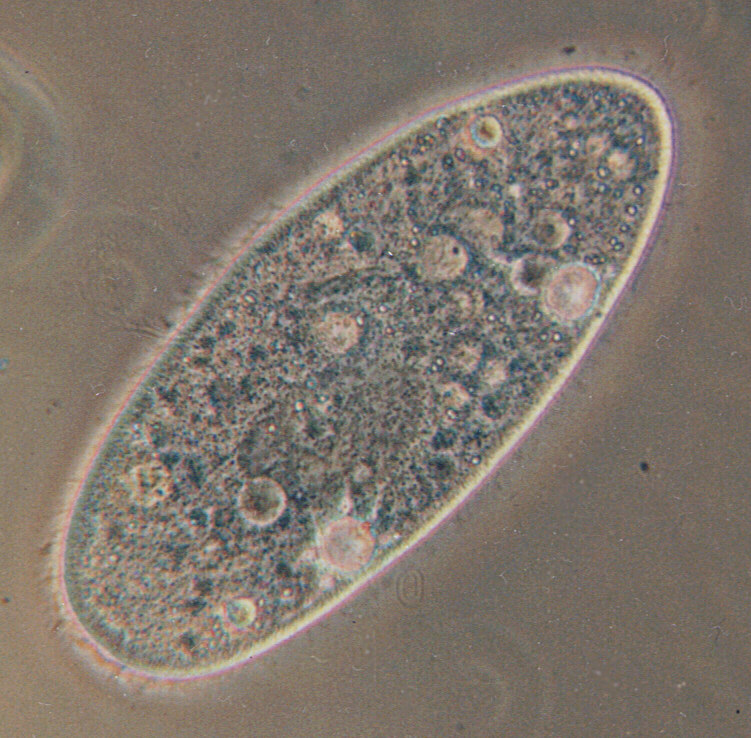
\includegraphics[width=0.97\textwidth]{Figures/Paramecium.jpg}
    \caption{Picture of a paramecium. \cite{wikipedia}}
    \label{fig:paramecium}
    \end{figure}
\end{minipage}

\noindent
\begin{minipage}{0.49\textwidth}

\vspace{1.2em}

\subsection{Galvanotaxis}
There are four reactions possible when an electric field is applied to paramecium:

\begin{itemize}
    \item No response
    \item Ciliary reversal
    \item Cell's contraction
    \item Cell's death
\end{itemize}

Figure \textbf{\ref{fig:cell_response}} shows how cells react to the electric field as a function of the pulse strength and duration.

\end{minipage}
\hfill
\begin{minipage}{0.49\textwidth}
    \begin{figure}[H]
    \centering 
    \captionsetup{width=0.9\linewidth, justification=centering}
    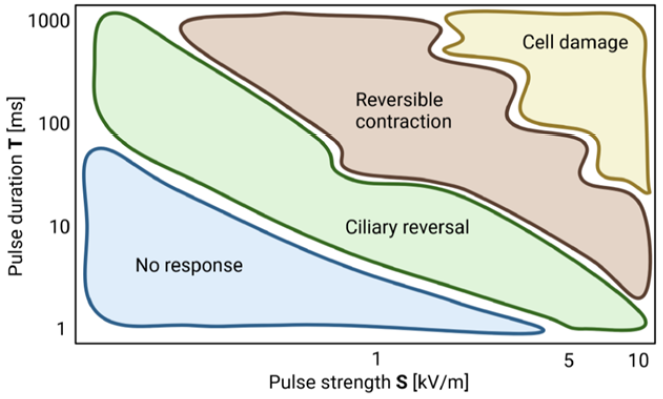
\includegraphics[width=1\textwidth]{Figures/Cell_response.png}
    \caption{Paramecium's response as a function of the pulse strength and duration. \cite{Notice}}
    \label{fig:cell_response}
    \end{figure}
\end{minipage}



\subsection{Ciliary reversal}

Paramecium responds to an external electric field by reversing the direction of its ciliary beating, a phenomenon known as ciliary reversal. Under normal conditions, the cilia beat in a coordinated pattern from front to back, propelling the organism forward. However, when the anterior end of the cell is exposed to a cathodal electric field, the membrane depolarizes, causing voltage-gated calcium channels to open and \ce{Ca^2+} ions to enter the cell. This calcium influx triggers a reversal in the ciliary beat direction, making the Paramecium swim backward. When an electric field is constantly applied, the ciliary reversal is such that the paramecium aligns with the E-field and swims towards the cathode. This response is part of the cell’s natural avoidance behavior, allowing it to reorient itself away from potentially harmful stimuli. The reversal is rapid and temporary, and once the membrane repolarizes, forward swimming resumes. \cite{naitoh1972}



\subsection{Contraction, trichocysts expulsion and death}

Paramecium exhibits a rapid contraction response when exposed to an external electric field, a phenomenon often referred to as electroshock response. When a strong enough electric stimulus is applied, the membrane becomes depolarized, causing a sudden influx of calcium ions into the cell. This triggers a rapid and temporary contraction of the cell body, often accompanied by the expulsion of trichocysts and a brief halt in movement. The response is thought to be protective, as it allows the organism to quickly react to sudden environmental changes. After the stimulus ends, the cell returns to its normal shape and resumes swimming. If the electric field is too strong or prolonged, it can lead to irreversible damage or death of the cell. \cite{naitoh1969}

\noindent
\begin{minipage}{0.57\textwidth}
    Paramecium uses specialized organelles called trichocysts as a rapid defense mechanism. These elongated, capsule-like structures are embedded in the outer layer of the cell and can be explosively discharged in response to mechanical or chemical stimuli. Upon activation, each trichocyst releases a thin, filamentous thread that shoots out through the cell membrane, forming a spiky barrier around the organism. This process is believed to deter predators and is not harmful or toxic, but rather a passive defense strategy. Trichocysts can entangle or immobilize the cell itself or other cells, which can be useful in the case of predation. Trichocyst expulsion occurs rapidly (few ms) and does not require energy, relying instead on physical and ionic changes within the cell. \cite{hausmann2003}. An image of paramecium tricocysts is shown in \textbf{Figure \ref{fig:trichocysts}}.
    
\end{minipage}
\hfill
\begin{minipage}{0.4\textwidth}
    \begin{figure}[H]
    \centering 
    \captionsetup{width=1\linewidth, justification=centering}
    \includegraphics[width=1\textwidth]{TP6 dying cells/Figures/trichocysts.png}
    \caption{Paramecium trichocysts \cite{trichocysts}}
    \label{fig:trichocysts}
    \end{figure}
\end{minipage}
\noindent
\subsection{Experimental method}

The experiment consists in analyzing the movement of paramecium in different media and their response to an applied electric field.

\subsubsection{Cells and media}

Paramecium are cultured in a medium of MilliQ. This medium is used to observe the paramecium in a controlled environment. For the second medium, a solution of \ce{Ca^2+} is added to the MilliQ water. The calcium ions modify the osmotic pressure of the medium, which influences the movement of the paramecium and their response to the electric field.

\subsubsection{Chamber}

To observe paramecium, they are placed in a chamber. It consists of a glass slide with two thin copper foils on each side, which are used to apply the electric field. A coverslip is placed on top to create a thin volume between the slide and the coverslip. A layer scheme of the chamber is shown in figure \textbf{\ref{fig:Chamber_layer}} and a scheme of the chamber seen from the top is shown in figure \textbf{\ref{fig:Chamber_top}}. The distance between the two copper foils (width of the chamber) is 5mm. 

\noindent
\begin{minipage}{0.49\textwidth}
    \begin{figure}[H]
    \centering 
    \captionsetup{width=0.9\linewidth, justification=centering}
    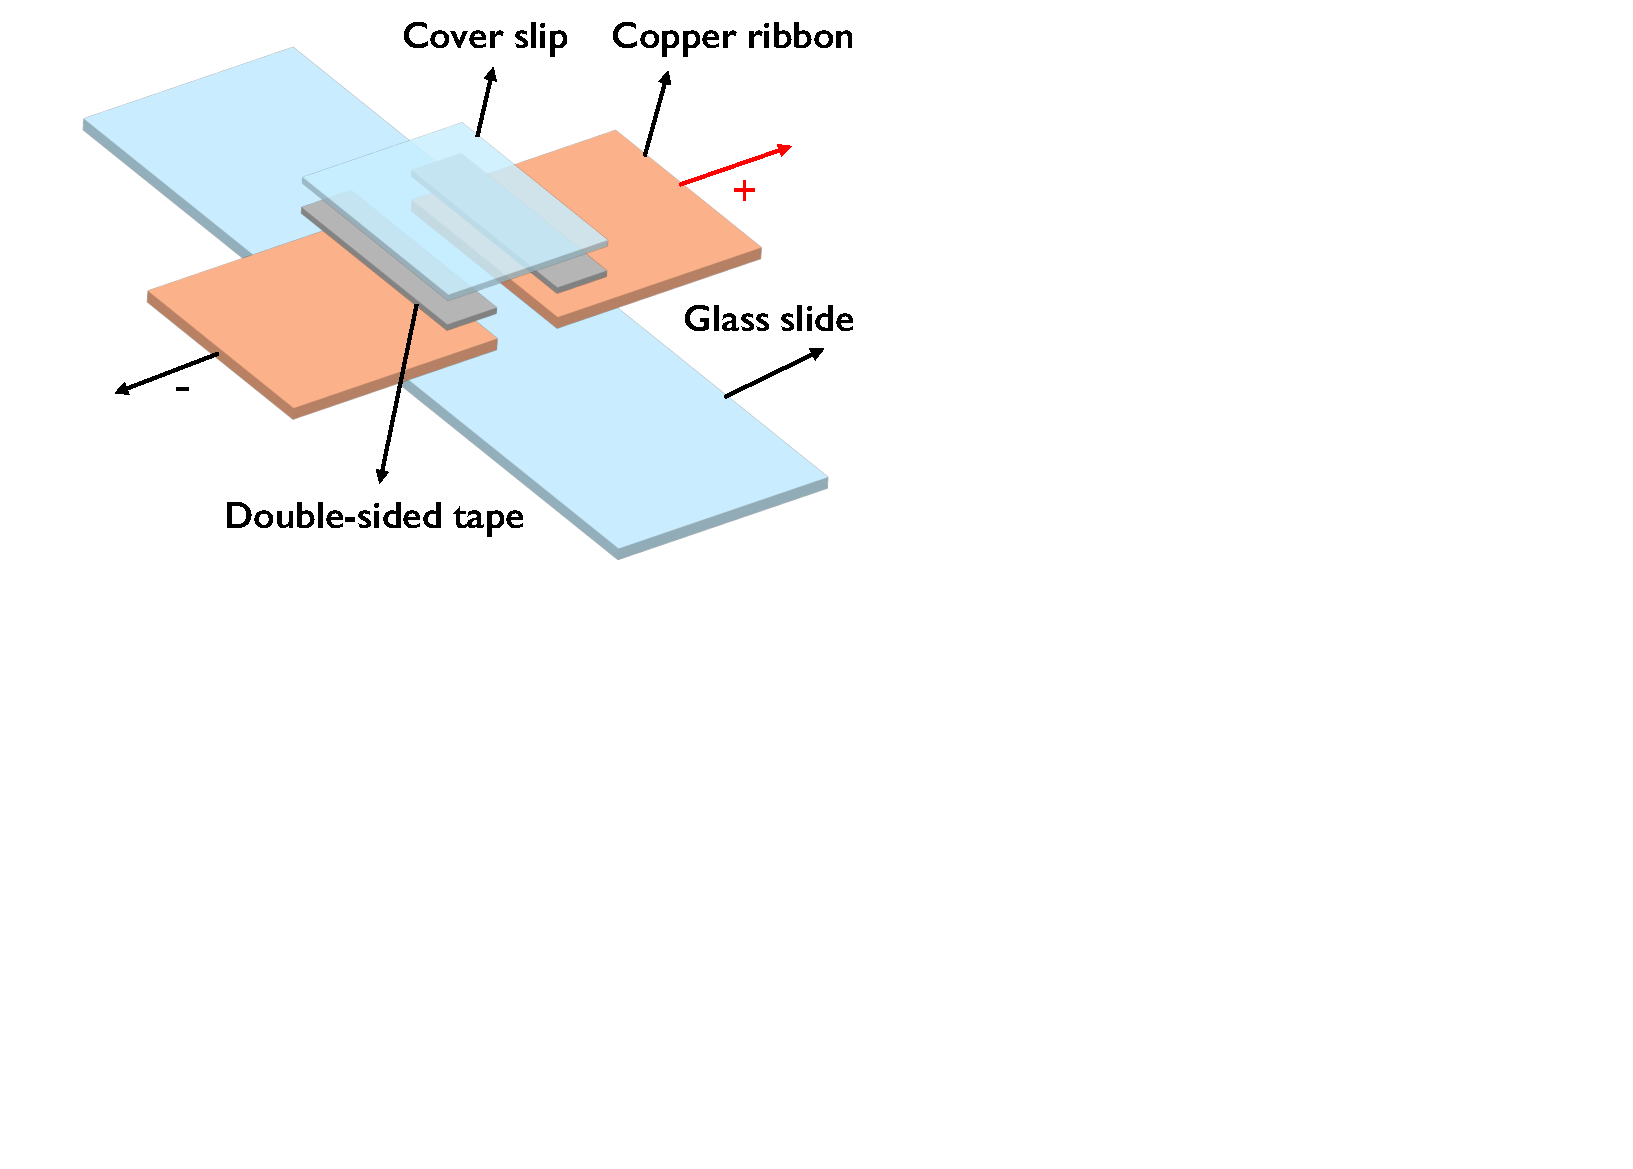
\includegraphics[width=0.9\textwidth]{Figures/Chamber_layer.pdf}
    \caption{Layer scheme of the chamber.}
    \label{fig:Chamber_layer}
    \end{figure}
\end{minipage}
\hfill
\begin{minipage}{0.49\textwidth}
    \begin{figure}[H]
    \centering 
    \captionsetup{width=0.9\linewidth, justification=centering}
    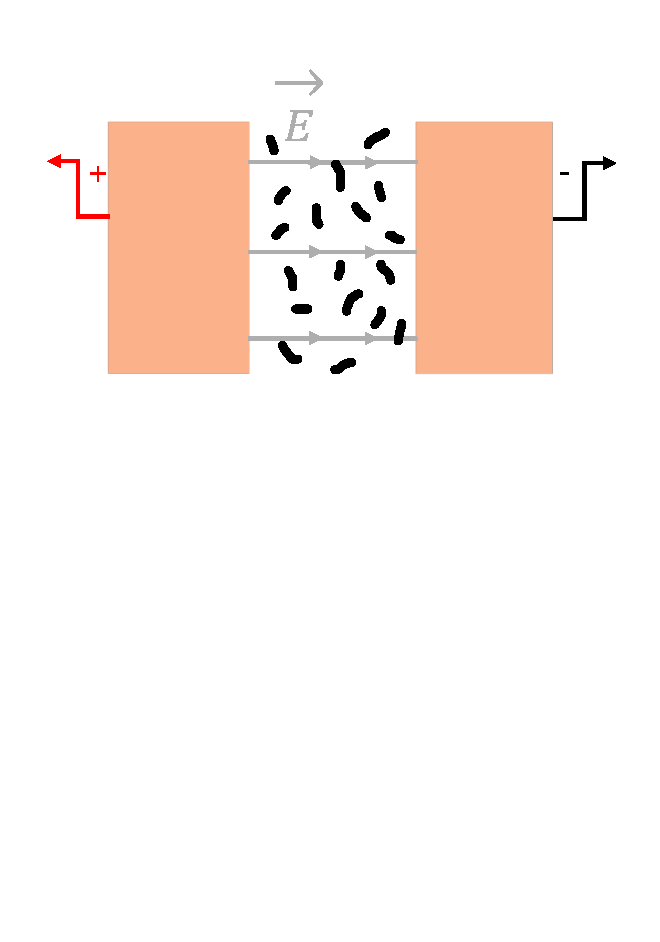
\includegraphics[width=0.9\textwidth]{Figures/Chamber_top.pdf}
    \caption{Scheme of the chamber seen from the top.}
    \label{fig:Chamber_top}
    \end{figure}
\end{minipage}

\subsubsection{Observation and electric pulse}

Paramecium are observed with an optical microscope. Using the microscope's program, the movement of cells can be recorded in short videos which can be exported for analysis. The electric field is applied to the chamber by connecting the copper foils to a control box. The control box allows to chose the pulse strength and duration, and is connected to a generator. A picture of the experimental setup is shown in figure \textbf{\ref{fig:setup}}.
\begin{figure}[H]
\centering 
\captionsetup{width=0.9\linewidth, justification=centering}
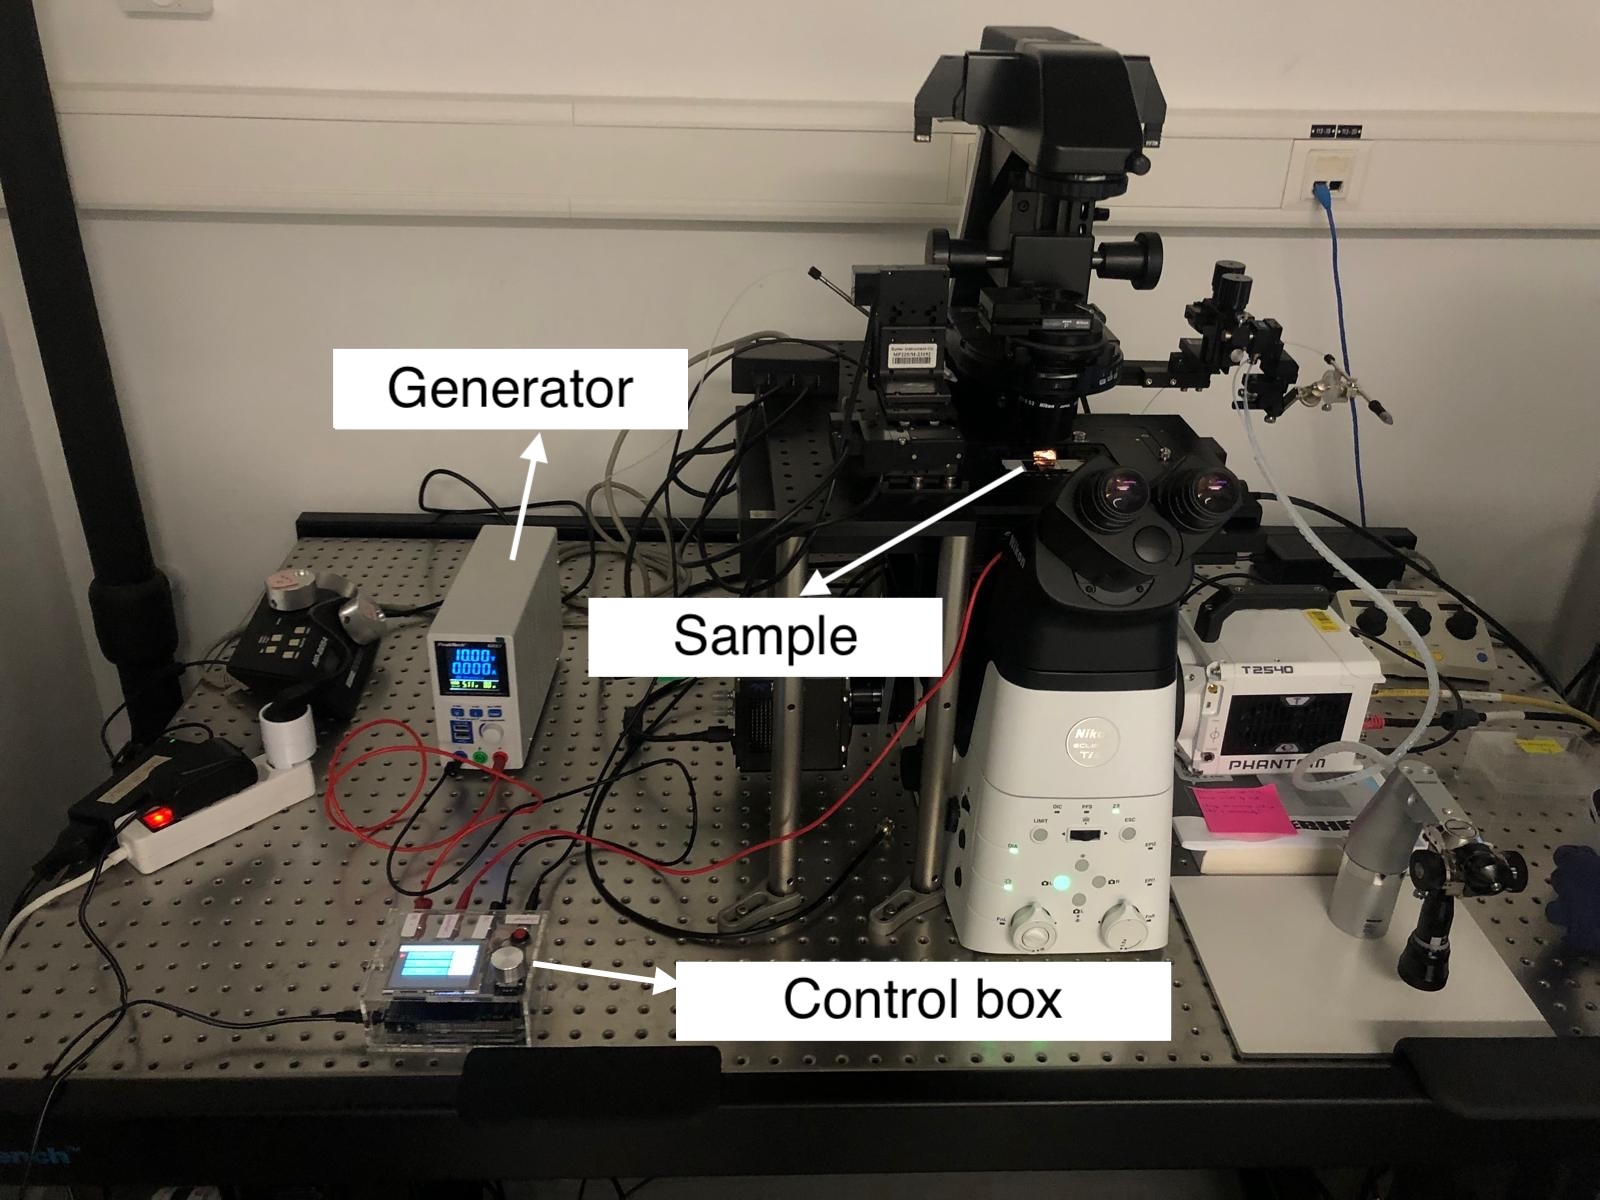
\includegraphics[width=0.7\textwidth]{Figures/gros_setup.jpeg}
\caption{Experimental setup}
\label{fig:setup}
\end{figure}    
The pulse duration is set to 1000ms and the different pulse voltages used in the experiment are 0V (no pulse), 5V, 10V, 15V and 20V, corresponding to pulse strrengths of 0V/mm, 1V/mm, 2V/mm, 3V/mm and 4V/mm respectively. The pulse is applied to the chamber while the video is being recorded. 

\subsection{Data analysis}

\begin{minipage}{0.49\textwidth}
The videos were processed to extract the data using the Fiji software with the TrackMate plugin. This tool tracks cells frame by frame and records their positions as a function of time. An example of the final output from this processing is shown in \textbf{Figure~\ref{fig:trackmate}}.

However, a technical issue during video capture with the microscope introduced lag and noise into the extracted data. To mitigate this, the cell trajectories over time were smoothed using a moving average technique. While effective in reducing noise, this method may also lead to the loss of certain details, such as brief fluctuations in speed or changes in direction.
\end{minipage}
\hfill
\begin{minipage}{0.47\textwidth}
\begin{figure}[H]
\centering 
\captionsetup{width=1\linewidth, justification=centering}
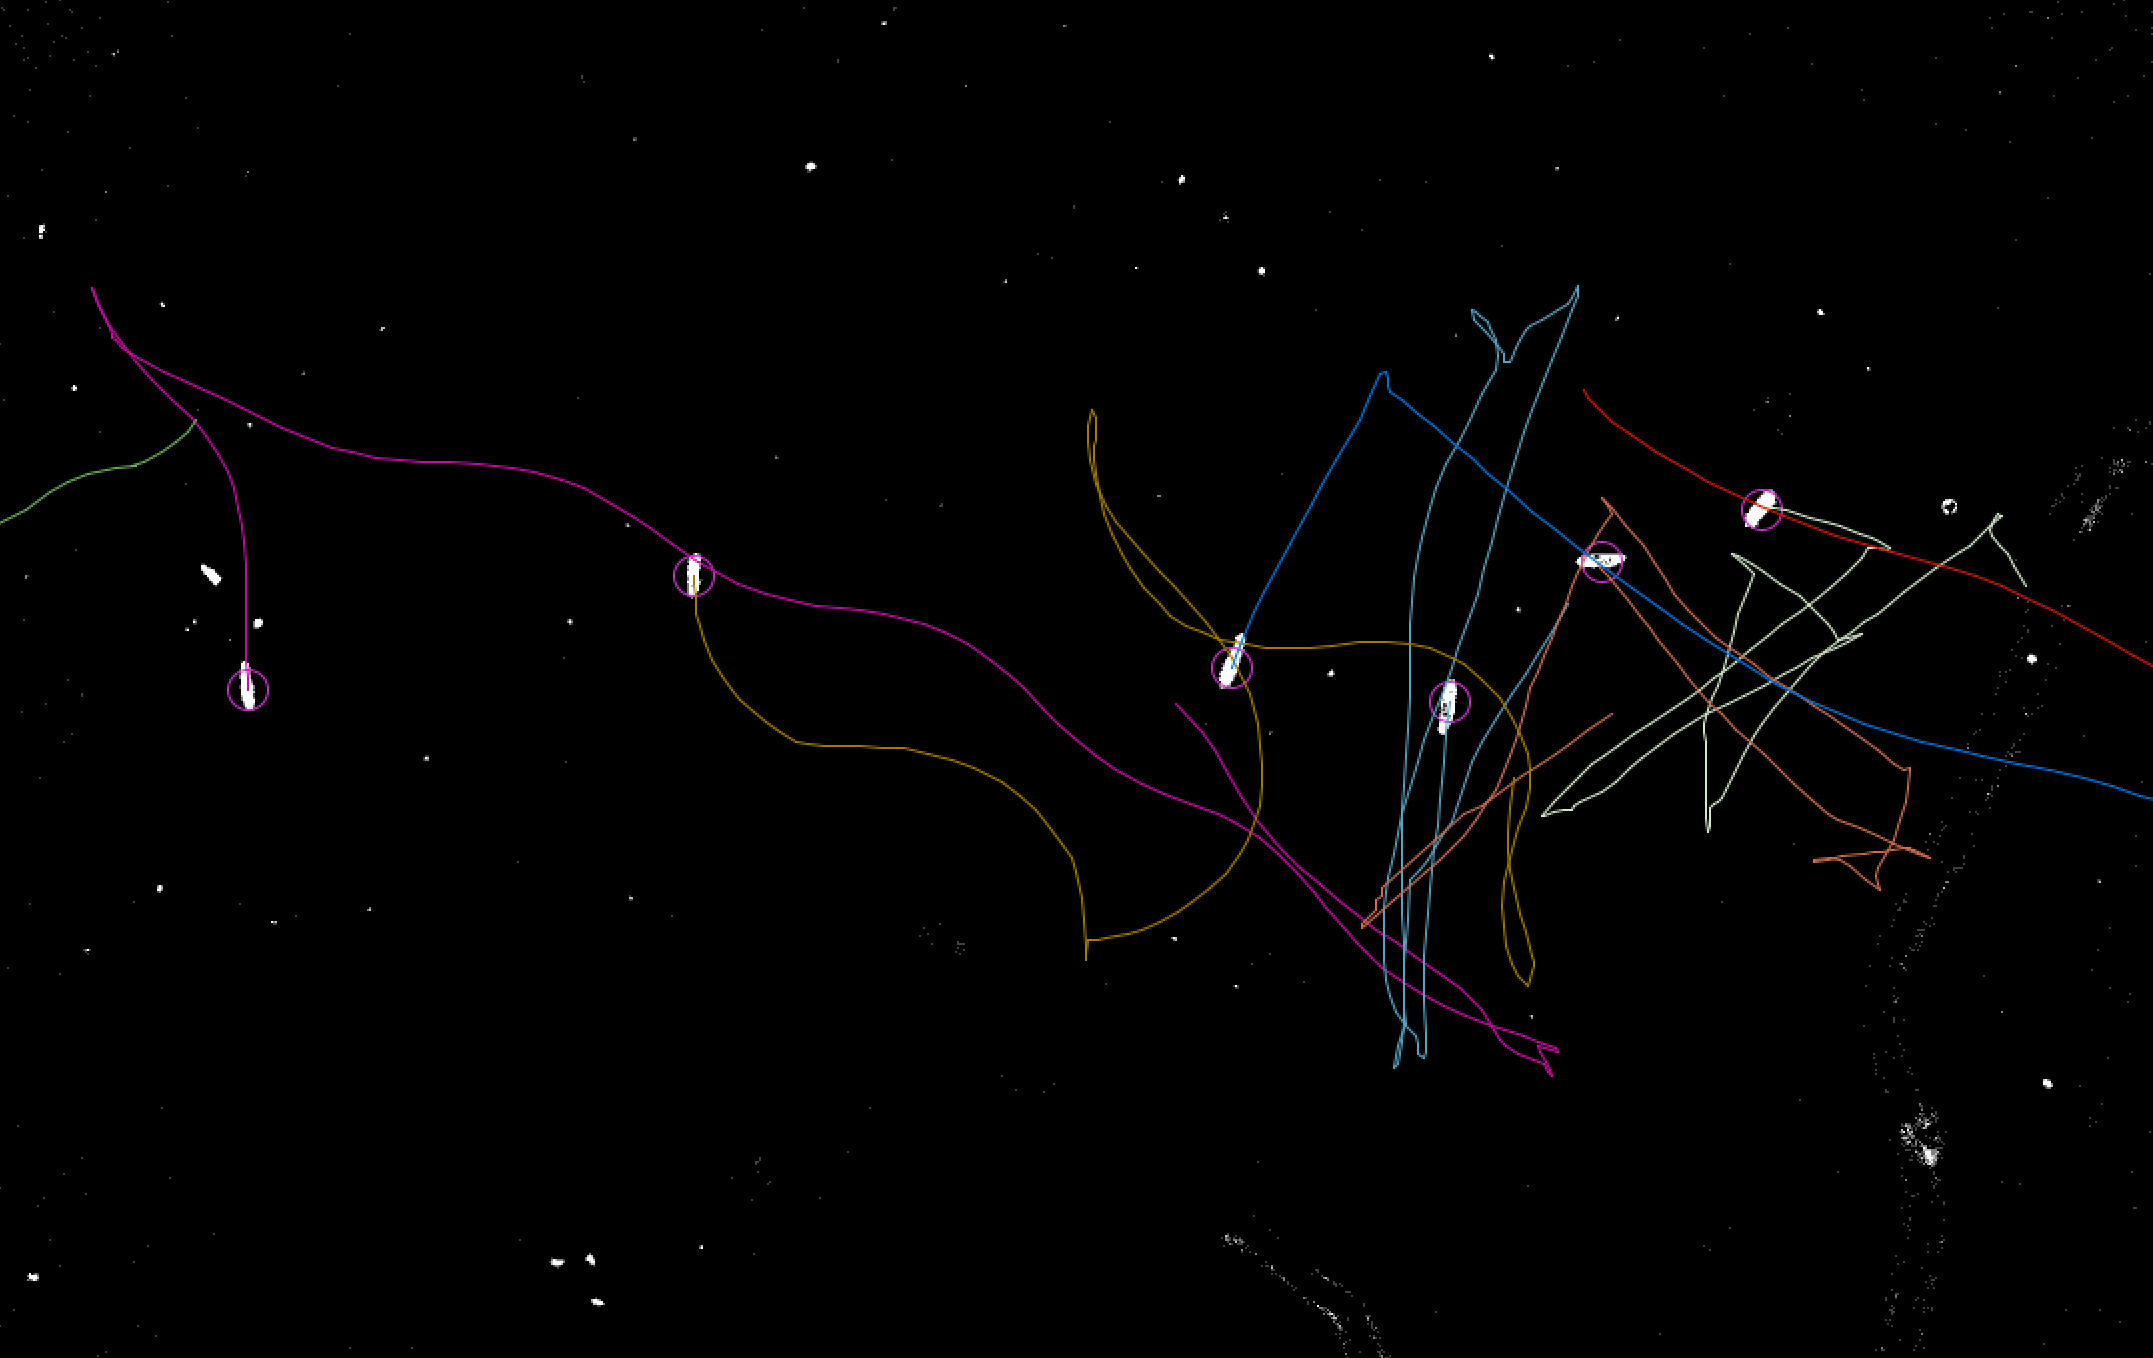
\includegraphics[width=0.9\textwidth]{Figures/Fiji.png}
\caption{Example of a video processed with TrackMate. The white cylinders are the cells and the different trajectories are highlighted in different colors.}
\label{fig:trackmate}
\end{figure}
\end{minipage}


\section{Results and analysis}

\subsection{Qualitative analysis}

\paragraph{MQ vs Ca medium}
The paramecia in the \ce{Ca^2+} medium exhibit greater sensitivity to the applied electric field; specifically, their velocity norm changes more compared to those  in the MilliQ medium. This higher sensitivity will be confirmed through quantitative analysis. Furthermore, a higher number of damaged or dead paramecia are observed in the \ce{Ca^2+} medium following exposure to strong electric field pulses (15V and 20V). This is attributed to the higher ion density surrounding the paramecia in this medium, which leads to an increased ion flux into the cells and higher response

\paragraph{Ciliary reversal}
The first noticeable effect is that the paramecia change their direction of movement upon application of the electric pulse. This behavior is illustrated in \textbf{Figures~\ref{fig:before_pulse}} and \textbf{\ref{fig:after_pulse}}, which show the positions of the paramecia immediately before and after the application of a 20V pulse. This reversal of direction is a clear indication of ciliary reversal.

\noindent
\begin{minipage}{0.49\textwidth}
\begin{figure}[H]
\centering 
\captionsetup{width=0.9\linewidth, justification=centering}
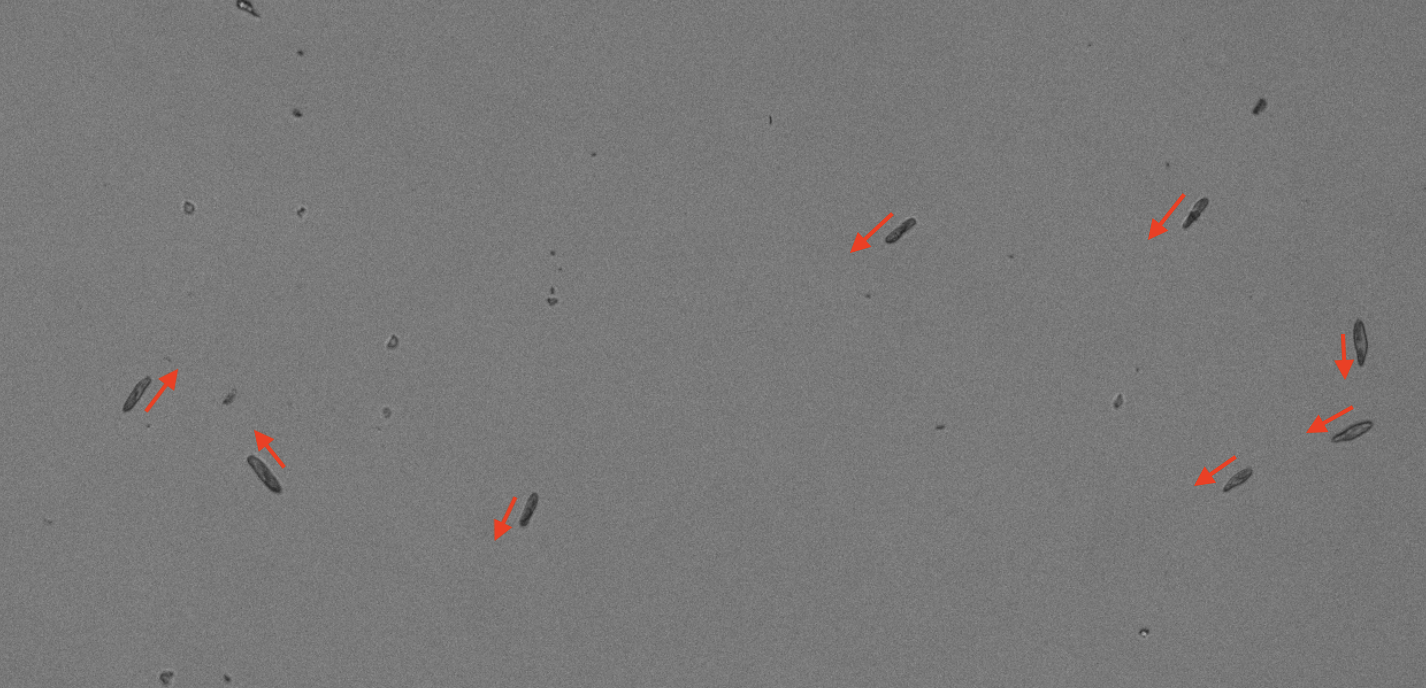
\includegraphics[width=0.9\textwidth]{Figures/before_pulse.png}
\caption{Paramecia just before the application of the pulse.}
\label{fig:before_pulse}
\end{figure}
\end{minipage}
\hfill
\begin{minipage}{0.49\textwidth}
\begin{figure}[H]
\centering 
\captionsetup{width=0.9\linewidth, justification=centering}
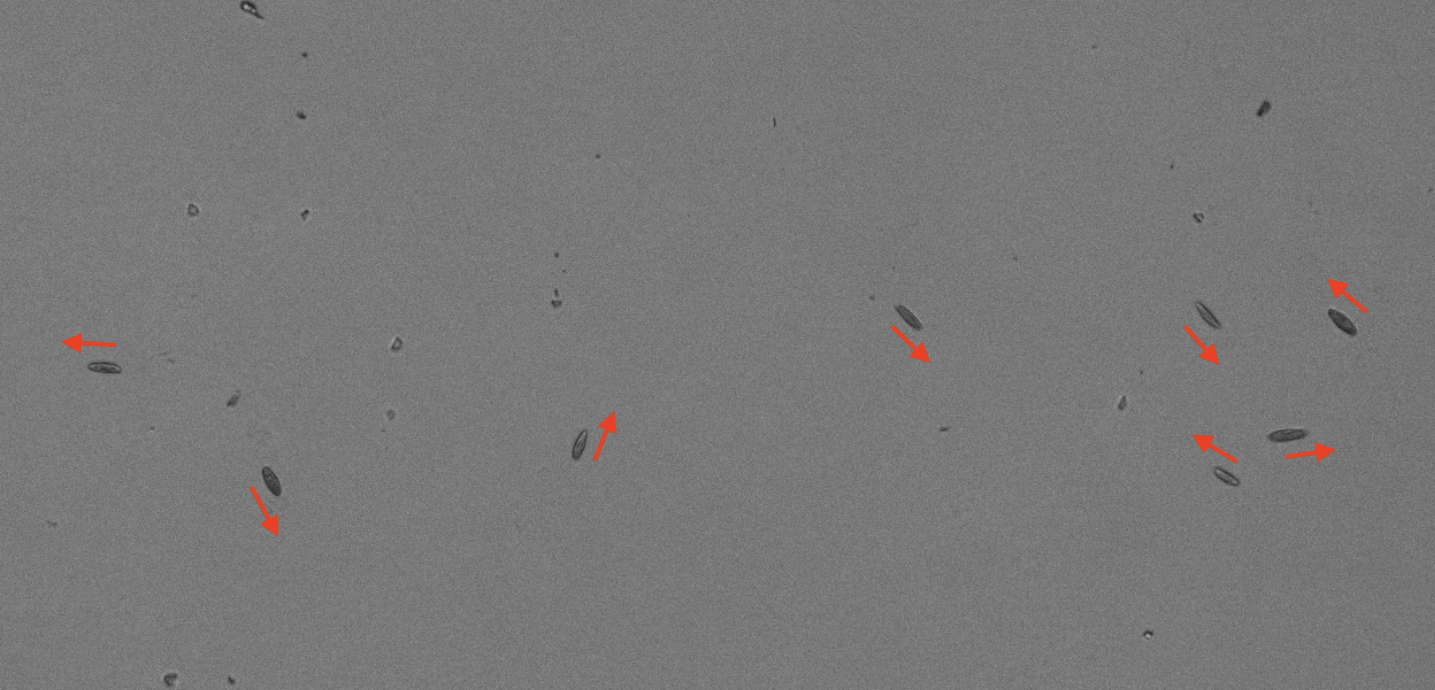
\includegraphics[width=0.9\textwidth]{Figures/after_pulse.png}
\caption{Paramecia just after the application of the pulse.}
\label{fig:after_pulse}
\end{figure}
\end{minipage}



\paragraph{Aligning in opposition with the electric field}

After ciliary reversal, the paramecia adjust their direction of movement to to the electric field, as long as the pulse is applied. The relatively long pulse duration used in the experiment (1000ms) enabled this behavior to be clearly observed. This alignment is more pronounced at lower voltages (5V and 10V) than at higher voltages (15V and 20V). A plausible explanation is that at higher voltages, the ciliary reversal is too strong, preventing the cells from relaxing and reorienting in time to align with the field.

For the MilliQ medium and a pulse strength of 1V/mm, the alignement is shown in \textbf{Figure \ref{fig:aligning_before}} and \textbf{\ref{fig:aligning_during_pulse}}. The video from which these figures were extracted is available on youtube and can be seen by scanning the QR-code in \textbf{Figure \ref{fig:Paramecium_aligning}} in the appendix. 

\noindent
\begin{minipage}{0.49\textwidth}
\begin{figure}[H]
\centering 
\captionsetup{width=0.9\linewidth, justification=centering}
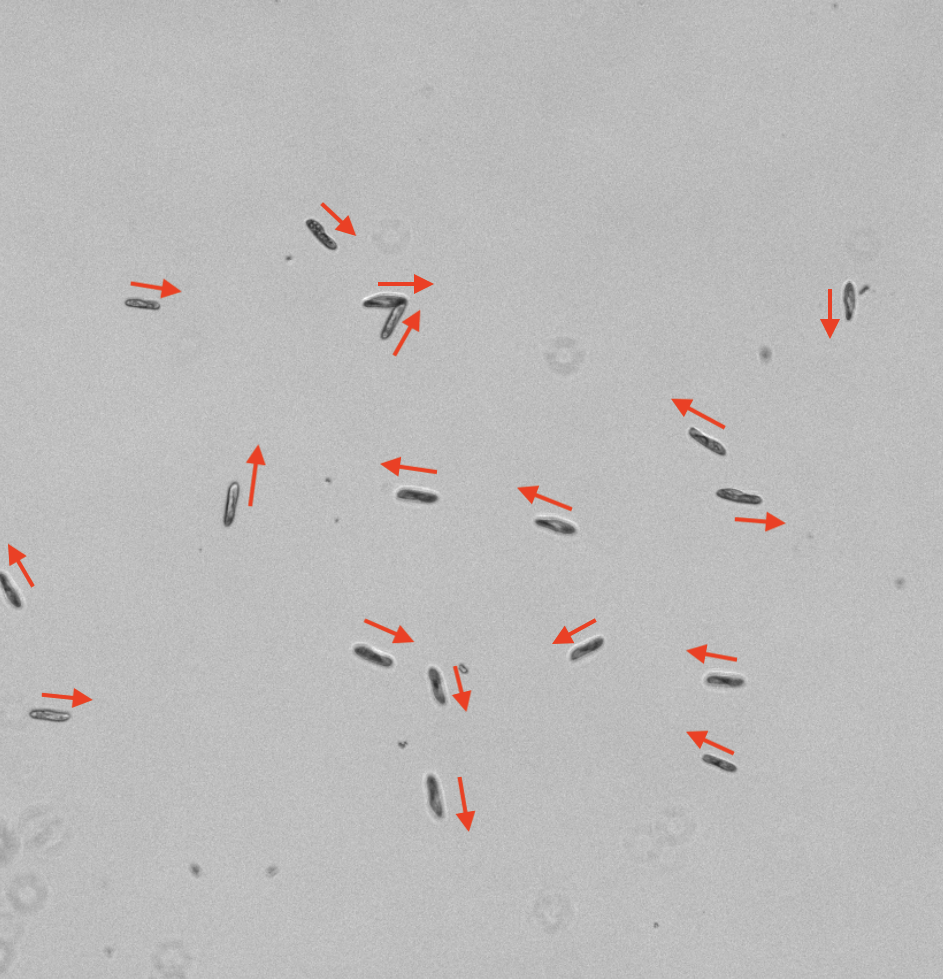
\includegraphics[width=0.8\textwidth]{Figures/aligning_before.png}
\caption{Paramecia just before the application of the pulse, pointing in different directions.}
\label{fig:aligning_before}
\end{figure}
\end{minipage}
\hfill
\begin{minipage}{0.49\textwidth}
\begin{figure}[H]
\centering 
\captionsetup{width=0.9\linewidth, justification=centering}
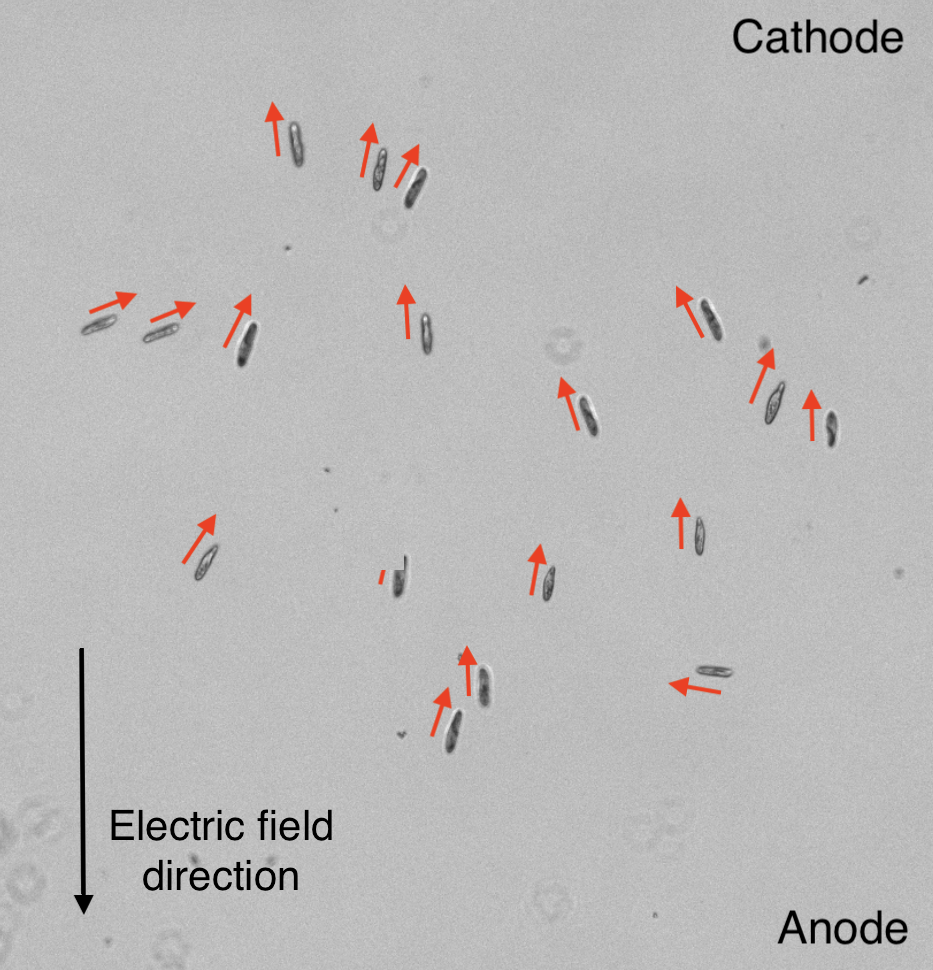
\includegraphics[width=0.8\textwidth]{Figures/aligning_during_pulse.png}
\caption{Paramecia just after the application of the pulse, aligning in the opposite direction of the electric field.} 
\label{fig:aligning_during_pulse}
\end{figure}
\end{minipage}

\paragraph{Contraction and trichocysts expulsion}
At high pulse strengths (15 V and 20 V), cell contraction can be observed. The contraction process for three different cells exposed to multiple consecutive 15 V pulses in MilliQ medium is illustrated in \textbf{Figure \ref{fig:Cell_in_contraction_1}}, with their state a few minutes later shown in \textbf{Figure \ref{fig:Cell_in_contraction_2}}. Additionally, a video documenting this phenomenon is available on YouTube and can be accessed by scanning the QR code in \textbf{Figure \ref{fig:Cells_contracting}} in the appendix. A fully contracted cell from the same sample, captured at higher resolution, is displayed in \textbf{Figure \ref{fig:Contracted_cell}}.

\noindent
\begin{minipage}{0.49\textwidth}
\begin{figure}[H]
\centering 
\captionsetup{width=0.9\linewidth, justification=centering}
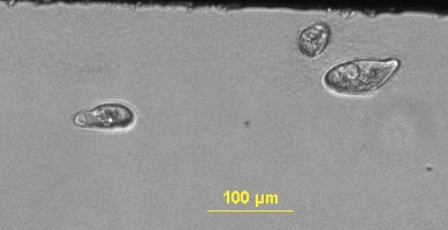
\includegraphics[width=0.9\textwidth]{Figures/Cells_in_contraction_1.png}
\caption{Paramecia in contraction.}
\label{fig:Cell_in_contraction_1}
\end{figure}
\end{minipage}
\hfill
\begin{minipage}{0.49\textwidth}
\begin{figure}[H]
\centering 
\captionsetup{width=0.9\linewidth, justification=centering}
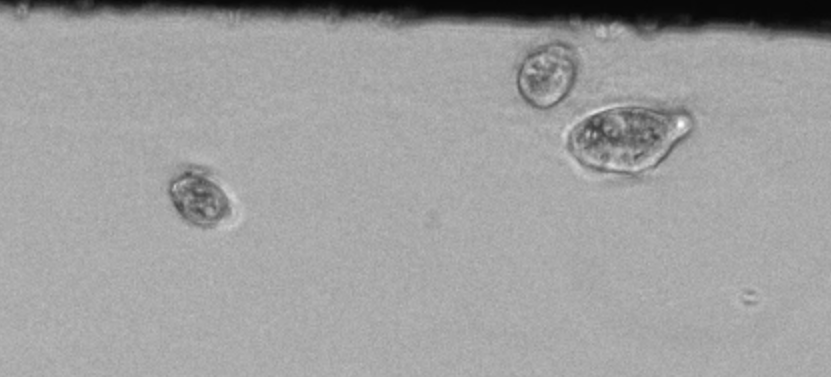
\includegraphics[width=0.9\textwidth]{Figures/Cells_in_contraction_2.png}
\caption{Paramecia in contraction after a couple of minutes.}
\label{fig:Cell_in_contraction_2}
\end{figure}
\end{minipage}
In the video, the movement of the cytoskeleton in one paramecium can be directly observed. The cilia of this cell are beating rapidly but in a disorganized manner, indicating cellular damage. Because the cilia cannot beat properly, the cell is unable to swim. As described in the theory section, both contraction and ciliary disorganization are responses to the applied electric field.

Within the same sample, some paramecia expelled their trichocysts and became stationary or spinning around their longitudinal axis. An example of a paramecium expelling trichocysts while spinning is shown in \textbf{Figure \ref{fig:Trichocysts_expulsion}}. A video capturing this process in two other paramecia is available on YouTube and can be accessed by scanning the QR code in \textbf{Figure \ref{fig:Swimming_Damaged_Paramecium}} in the appendix.

\noindent
\begin{minipage}{0.49\textwidth}
\begin{figure}[H]
\centering 
\captionsetup{width=0.9\linewidth, justification=centering}
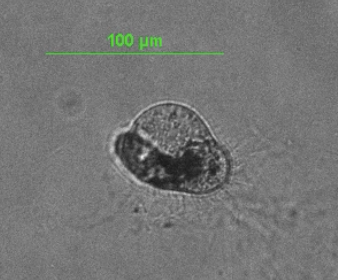
\includegraphics[width=0.9\textwidth]{Figures/Contracted_cell.png}
\caption{Contracted paramecium}
\label{fig:Contracted_cell}
\end{figure}
\end{minipage}
\hfill
\begin{minipage}{0.49\textwidth}
\begin{figure}[H]
\centering 
\captionsetup{width=0.9\linewidth, justification=centering}
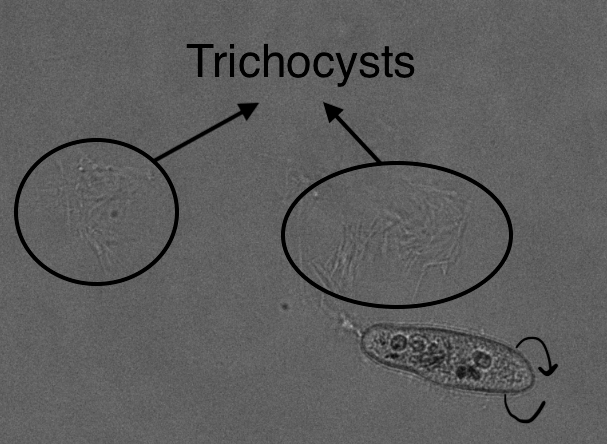
\includegraphics[width=0.9\textwidth]{Figures/Trichocysts_expulsion.png}
\caption{Paramecium expelling trichocysts while spinning along its longitudinal axis.}
\label{fig:Trichocysts_expulsion}
\end{figure}
\end{minipage}

Trichocyst expulsion reflects an excessive ionic flux across the cell membrane, to which the paramecium reacts by expelling these organelles (see theory). In these cases, the ionic flux caused important damages to the cells, making them unable to swim properly. Some cells may also me stuck in their own trichocysts, this is the case of one of the paramecia in the video (\textbf{Figure \ref{fig:Swimming_Damaged_Paramecium}}).

\paragraph{Relaxation of the Cells}
As mentioned in previous sections, cells exhibit various responses to the application of an electric pulse. Some of these responses are reversible, meaning the cells return to their original state after a certain relaxation period. This is observed in phenomena such as ciliary reversal and the temporary increase in swimming speed following pulse application. The (non-damaged) cells typically return to their normal speed within a few seconds after the pulse. Although reversible contraction was not observed in this experiment, it is a known reversible process reported in the literature.

\subsection{Quantitative analysis}

\noindent
\begin{minipage}{0.39\textwidth}

    \paragraph{Trajectories of paramecium}
    
    As explained in the theory section, paramecium typically move along one of three main types of trajectories: linear, helicoidal, or circular. \textbf{Figure \ref{fig:trajectories}} shows the different types of trajectories observed in the \ce{Ca^2+} medium without any electric stimulation. These were extracted from video recordings using the Fiji software with the TrackMate plugin. Each colored path corresponds to a different tracked cell. The presence of more circular and helicoidal motions in the Ca\textsuperscript{2+} dmedium suggests an effect of calcium ions on cell behavior even in the absence of electric fields. 

\end{minipage}
\hfill
\begin{minipage}{0.59\textwidth}
    \begin{figure}[H]
    \centering 
    \captionsetup{width=0.95\linewidth, justification=centering}
    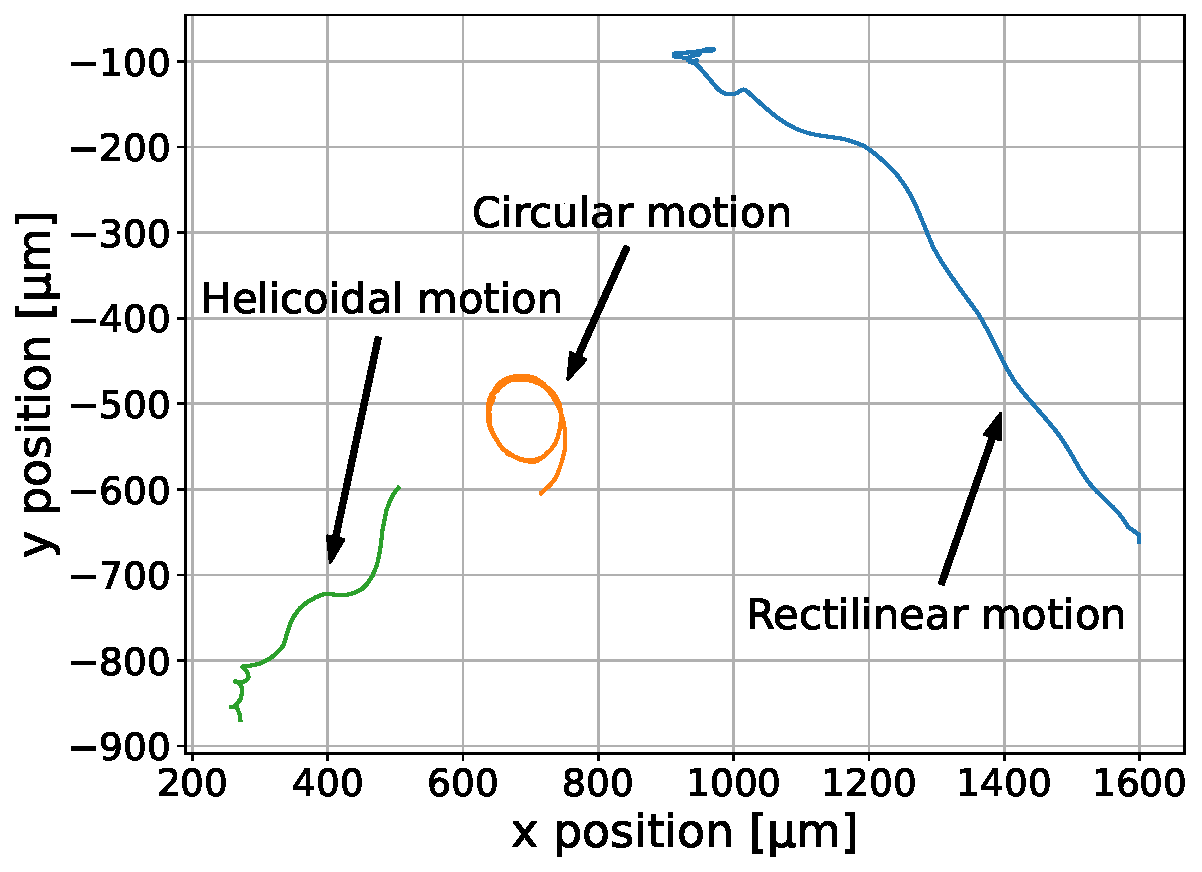
\includegraphics[width=0.9\textwidth]{Figures/2.5mM_0V_007_trajectories.pdf}
    \caption{Different type of paramecium trajectories in the \ce{Ca^2+} medium without electric pulse.}
    \label{fig:trajectories}
    \end{figure}
\end{minipage}

\paragraph{Electric pulse response}

Now, the response of Paramecium to the electric pulse is analyzed. The velocities of textit{Paramecium are plotted as a function of time for different voltages and for the MilliQ medium in \textbf{Figure \ref{fig:velocity_time_MQ_0V}},\textbf{Figure \ref{fig:velocity_time_MQ_5V}}},\textbf{Figure \ref{fig:velocity_time_MQ_10V}},\textbf{Figure \ref{fig:velocity_time_MQ_15V}} and \textbf{Figure \ref{fig:velocity_time_MQ_20V}}. Additionally, a box plot is presented for each voltage in \textbf{Figure \ref{fig:velocity_vs_voltage_MQ}}. These box plots are constructed using the time-averaged velocity of each cell over a 2-second interval following the application of the electric pulse. The same results are plotted for the \ce{Ca^2+} medium in \textbf{Figure \ref{fig:velocity_time_Ca_0V}},\textbf{Figure \ref{fig:velocity_time_Ca_5V}},\textbf{Figure \ref{fig:velocity_time_Ca_10V}},\textbf{Figure \ref{fig:velocity_time_Ca_15V}},\textbf{Figure \ref{fig:velocity_time_Ca_20V}} and \textbf{Figure \ref{fig:velocity_vs_voltage_Ca}}.
\begin{figure}[H]
    \centering
    \begin{minipage}[t]{0.49\textwidth}
        \centering
        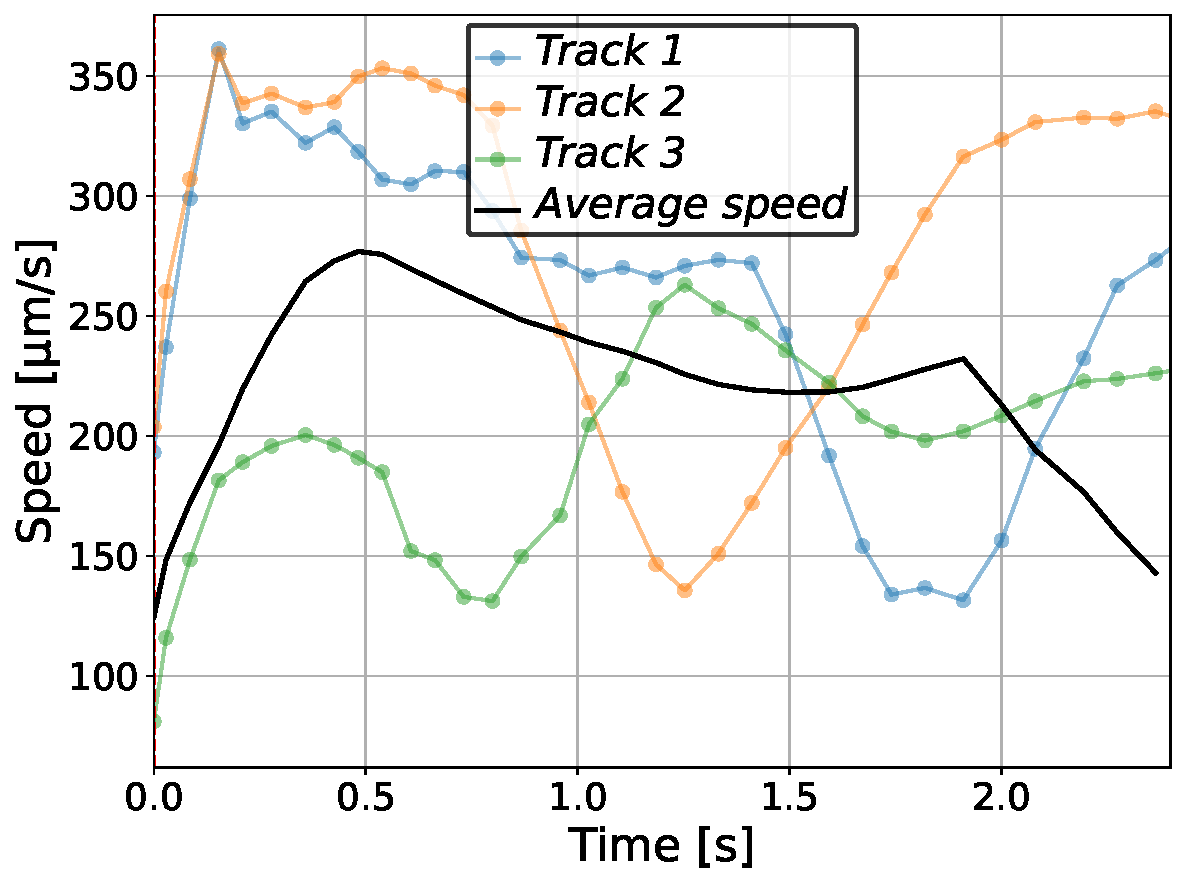
\includegraphics[width=0.95\textwidth]{Figures/MQ_0V_001_velocity_time.pdf}
        \caption{Velocity in MilliQ medium at 0V.}
        \label{fig:velocity_time_MQ_0V}
    \end{minipage}
    \hfill
    \begin{minipage}[t]{0.49\textwidth}
        \centering
        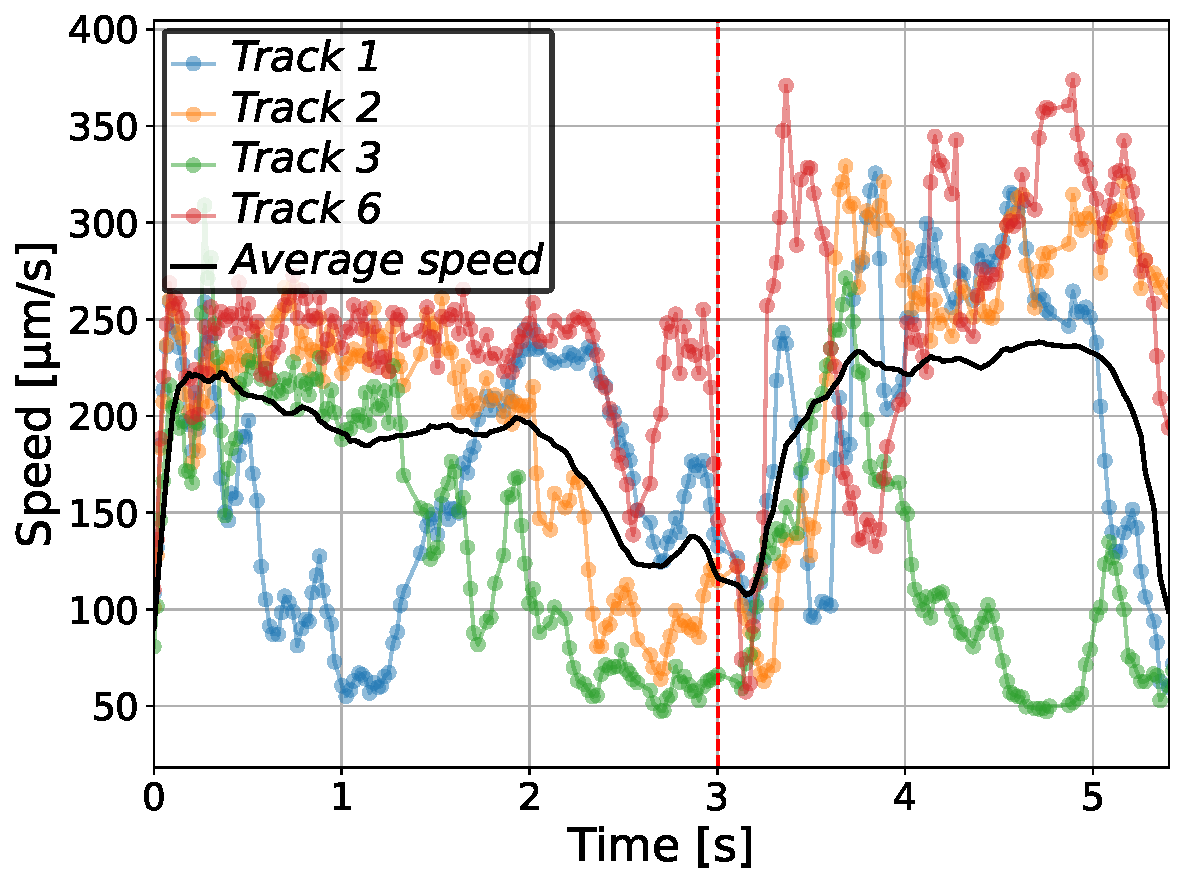
\includegraphics[width=0.95\textwidth]{Figures/MQ_5V_001_velocity_time.pdf}
        \caption{Velocity in MilliQ medium at 5V.}
        \label{fig:velocity_time_MQ_5V}
    \end{minipage}
\end{figure}

\begin{figure}[H]
    \centering
    \begin{minipage}[t]{0.49\textwidth}
        \centering
        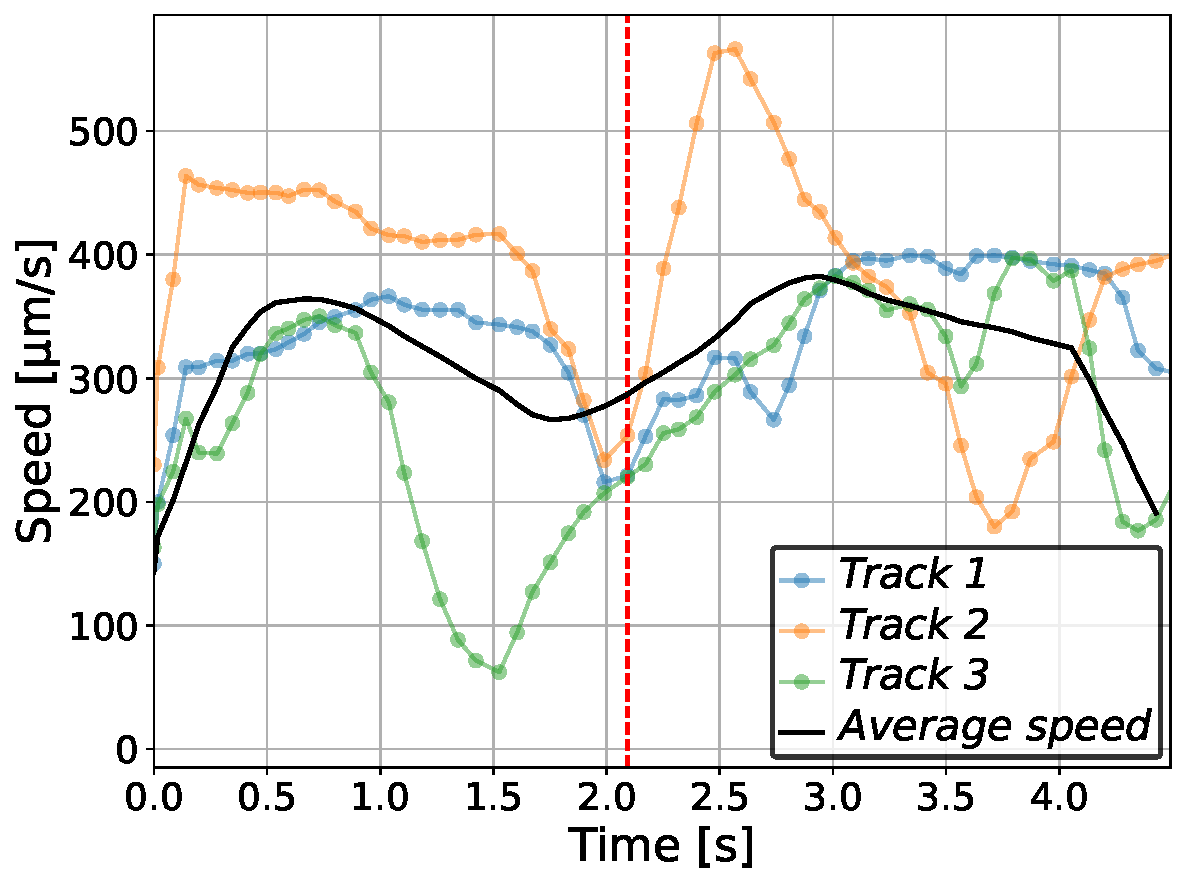
\includegraphics[width=0.95\textwidth]{Figures/MQ_10V_002_velocity_time.pdf}
        \caption{Velocity in MilliQ medium at 10V.}
        \label{fig:velocity_time_MQ_10V}
    \end{minipage}
    \hfill
    \begin{minipage}[t]{0.49\textwidth}
        \centering
        \includegraphics[width=0.95\textwidth]{Figures/MQ_15V_003_velocity_time.pdf}
        \caption{Velocity in MilliQ medium at 15V.}
        \label{fig:velocity_time_MQ_15V}
    \end{minipage}
\end{figure}

\begin{figure}[H]
    \centering
    \begin{minipage}[t]{0.49\textwidth}
        \centering
        \includegraphics[width=0.95\textwidth]{Figures/MQ_20V_velocity_time.pdf}
        \caption{Velocity in MilliQ medium at 20V.}
        \label{fig:velocity_time_MQ_20V}
    \end{minipage}
    \hfill
    \begin{minipage}[t]{0.49\textwidth}
        \centering
        \includegraphics[width=0.95\textwidth]{Figures/MQ_velocity_vs_voltage.pdf}
        \caption{Mean velocity vs voltage in MilliQ medium.}
        \label{fig:velocity_vs_voltage_MQ}
    \end{minipage}
\end{figure}


In the MilliQ medium and at 0V, the distribution of cell speeds is broad. The velocity of each individual cell varies over time, with multiple turning points observed in the velocity curves. These turning points correspond to directional changes in the cells’ trajectories. The range of velocities spans approximately from 140~$\mu$m/s to 350~$\mu$m/s.

Similar features—broad velocity distributions and frequent turning points—are observed for the 5V, 10V, 15V, and 20V pulses. Notably, immediately following the electric pulse, the velocity curves of individual cells often exhibit a change in slope, frequently marked by a turning point. This behavior is expected, as ciliary reversal typically occurs after the pulse, causing the cells to reorient in the direction opposite to the electric field. This sudden change in direction results in a brief deceleration.

A general trend can be seen in the mean velocity (averaged over all cells), which tends to increase following the application of the electric pulse. This increase is less pronounced and more gradual for the 10V and 15V pulses. Videos recorded for these conditions reveal that some cells reverse direction multiple times after the pulse, delaying the observable rise in global speed.

The box plots further illustrate these dynamics: the mean velocity slightly decreases for the 5V pulse compared to the 0V condition, then increases for the 10V, 15V, and 20V pulses. The mean velocities for the 10V, 15V, and 20V cases converge around 320~$\mu$m/s, suggesting a saturation effect in which the cells reach a maximum time-averaged speed following pulse application. It has to be noted that some cells achieve velocities up to 600~$\mu$m/s (see \textbf{Figure~\ref{fig:velocity_time_MQ_15V}}), which indicates the maximum time-averaged speed of the cells does not necessarily reflect the peak speed of individual cells.

The lower mean velocity observed at 5V compared to 0V may be attributed to a higher cell density in the 5V sample, resulting in increased cell–cell interactions and, consequently, a reduction in average speed.

For the 20V pulse, the velocity distribution is particularly broad. This likely reflects cellular damage in some individuals, which leads to significantly reduced velocities.

\begin{figure}[H]
    \centering
    \begin{minipage}[t]{0.49\textwidth}
        \centering
        \includegraphics[width=0.95\textwidth]{Figures/2.5mM_0V_007_velocity_time.pdf}
        \caption{Velocity in \ce{Ca^2+} medium at 0V.}
        \label{fig:velocity_time_Ca_0V}
    \end{minipage}
    \hfill
    \begin{minipage}[t]{0.49\textwidth}
        \centering
        \includegraphics[width=0.95\textwidth]{Figures/2.5mM_5V_003_velocity_time.pdf}
        \caption{Velocity in \ce{Ca^2+} medium at 5V.}
        \label{fig:velocity_time_Ca_5V}
    \end{minipage}
\end{figure}

\begin{figure}[H]
    \centering
    \begin{minipage}[t]{0.49\textwidth}
        \centering
        \includegraphics[width=0.95\textwidth]{Figures/2.5mM_10V_001_velocity_time.pdf}
        \caption{Velocity in \ce{Ca^2+} medium at 10V.}
        \label{fig:velocity_time_Ca_10V}
    \end{minipage}
    \hfill
    \begin{minipage}[t]{0.49\textwidth}
        \centering
        \includegraphics[width=0.95\textwidth]{Figures/2.5mM_15V_001_velocity_time.pdf}
        \caption{Velocity in \ce{Ca^2+} medium at 15V.}
        \label{fig:velocity_time_Ca_15V}
    \end{minipage}
\end{figure}

\begin{figure}[H]
    \centering
    \begin{minipage}[t]{0.49\textwidth}
        \centering
        \includegraphics[width=0.95\textwidth]{Figures/2.5mM_20V_001_velocity_time.pdf}
        \caption{Velocity in \ce{Ca^2+} medium at 20V.}
        \label{fig:velocity_time_Ca_20V}
    \end{minipage}
    \hfill
    \begin{minipage}[t]{0.49\textwidth}
        \centering
        \includegraphics[width=0.95\textwidth]{Figures/2.5mM_velocity_vs_voltage.pdf}
        \caption{Mean velocity vs voltage in \ce{Ca^2+} medium.}
        \label{fig:velocity_vs_voltage_Ca}
    \end{minipage}
\end{figure}


Similarly as for the MilliQ medium, the velocity distributions in the \ce{Ca^2+} medium are broad. Similar observations and comments can be made regarding the velocity increase and turning points in the velocity curves after the pulse.

The samples in this experiment 

It is also observed that the velocities of the cells before the application of the pulse tend to decrease with increasing voltage. This trend is not a direct effect of the voltage itself, but rather a consequence of the experimental procedure: the voltages were tested in increasing order, and the cell suspension was freshly prepared just prior to the 0V condition. As the experiments progressed, the cells spent more time in the \ce{Ca^{2+}} medium, allowing them to gradually adapt to this new environment. Over time, this adaptation led to a progressive reduction in their motility, eventually resulting in near-zero swimming speeds before pulse application.

The near-zero velocity observed in the \ce{Ca^{2+}} solution is a known phenomenon \cite{cell_stop} and is attributed to the high concentration of calcium ions in the medium. 



\vspace{1em}
Since the aim of this experiment is to study the response of cells under stress, the mean velocity (averaged over both cells and time) is computed within a time window defined by the relaxation time following the application of the electric pulse. It is worth noting (even without a formal statistical analysis) that the time between two directional changes of a cell is comparable to the relaxation time—that is, both are on the order of seconds. This suggests that the natural oscillations in cell speed, due to frequent directional changes, significantly contribute to the broadness of the velocity distribution.

To improve the statistical reliability of the measurements, one approach could be to reduce the natural frequency of directional changes. In this experiment, the high frequency of directional changes is likely a consequence of the small size of the observation chamber, which induces strong boundary effects. For future experiments, using a larger chamber could help mitigate these effects and yield more consistent velocity data.


Similarly as for the MilliQ medium, the velocity distributions in the \ce{Ca^2+} medium are broad. Similar observations and comments can be made regarding the velocity increase and turning points in the velocity curves after the pulse.

The samples of the \ce{Ca^2+} medium were prepared with a higher cell density than those of the MilliQ medium. This higher density causes the velocity distribution in the box plots to be narrower than in the MilliQ medium. 

For the 15V pulse, the velocity distribution is particularly broad, this is due to a high number of damaged cells with zero or near-zero velocities. It can be seen on \textbf{Figure~\ref{fig:velocity_time_Ca_15V}} that some cells have a velocity of 0~$\mu$m/s after the pulse, indicating that they are either dead or severely damaged. 

The tendancy of the mean velocity to increase with pulse strength is more pronounced and clear in the \ce{Ca^2+} medium than in the MilliQ medium. This can be explained by the higher sensitivity of the cells to the electric field in the \ce{Ca^2+} medium. Indeed, the \ce{Ca^2+} medium has a higher ionic concentration than the MilliQ medium, which increases the ionic flux across the cell membrane when an electric field is applied. This leads to a stronger response of the cells to the electric field. A plateau is also reached for the mean velocity at 15V and 20V.


It is also observed that the velocities of the cells before the application of the pulse tend to decrease with increasing voltage. This trend is not a direct effect of the voltage itself, but rather a consequence of the experimental procedure: the voltages were tested in increasing order, and the cell suspension was freshly prepared just prior to the 0V condition. As the experiments progressed, the cells spent more time in the \ce{Ca^{2+}} medium, allowing them to gradually adapt to this new environment. Over time, this adaptation led to a progressive reduction in their motility, eventually resulting in near-zero swimming speeds before pulse application.

The near-zero velocity observed in the \ce{Ca^{2+}} solution is a known phenomenon \cite{cell_stop} and is attributed to the high concentration of calcium ions in the medium. 

% \subsection{MSD and autocorrelation}
% Then, a statistical analysis can be performed on the data. One can compute the autocorrelation of the velocity as a function of the lag-time. The autocorrelation is defined as:
% \begin{equation}
%     C(\tau) = \langle \vec{v}(t) \cdot \vec{v}(t+\tau) \rangle_t
% \end{equation}
% where $\vec{v}(t)$ is the velocity at time $t$ and $\tau$ is the lag-time. In the case of this experiment, the autocorrelation is computed with the normalized velocities. The velocity autocorrelation function is a measure of how fast the direction of the velocity changes over time. If the autocorrelation function drops quickly, it indicates that the velocity direction changes rapidly and often, while a slow decay suggests that the velocity direction remains relatively stable over time.

% Then, one can compute the mean square displacement (MSD) of the paramecium as a function of time. The MSD is defined as:
% \begin{equation}
%     \text{MSD}(\tau) = \langle |\vec{r}(t+\tau) - \vec{r}(t)|^2 \rangle_t
% \end{equation}
% where $\vec{r}(t)$ is the position of the paramecium at time $t$ and $\tau$ is the lag-time. The MSD is a measure of how far, on average, a particle moves from its initial position over time.



\section{Conclusion}

This experiment provided a systematic exploration of Paramecium’s responses to electric field stimulation under varying medium conductivities and voltage intensities. By analyzing both qualitative behaviors—such as ciliary reversal, alignment with the electric field, and contraction—and quantitative metrics like velocity distributions, we were able to identify distinct regimes of cellular response. The Ca²⁺-enriched medium was shown to enhance the cells' sensitivity to electrical pulses, leading to more pronounced effects and a higher incidence of irreversible damage at high voltages. Despite some experimental limitations, such as chamber size and potential adaptation effects, the data clearly demonstrated that the strength of the electrical stimulus and the ionic environment play critical roles in shaping Paramecium’s electromechanical behavior. These findings contribute to a better understanding of bioelectric signaling in unicellular organisms and open the way for further studies using more refined control over medium composition and electric pulse parameters.




\section{Annexes}

\begin{minipage}{0.49\textwidth}
\begin{figure}[H]
\centering 
\captionsetup{width=0.98\linewidth, justification=centering}
\includegraphics[width=0.9\textwidth]{Figures/Paramecium_aligning.png}
\caption{QR-code of the video of paramecium aligning in the opposite direction of the electric field. Link: \url{https://youtube.com/shorts/cjV4M5JLck4}}
\label{fig:Paramecium_aligning}
\end{figure}
\end{minipage}
\hfill
\begin{minipage}{0.49\textwidth}
\begin{figure}[H]
\centering 
\captionsetup{width=0.98\linewidth, justification=centering}
\includegraphics[width=0.9\textwidth]{Figures/Swimming_Damaged_Paramecium.png}
\caption{QR-code of the video of a damaged paramecium stuck in its own trichocysts and another damaged paramecium spinning along its longitudinal axis. Link: \url{https://youtube.com/shorts/yF_vT8V6dA8}}
\label{fig:Swimming_Damaged_Paramecium}
\end{figure}
\end{minipage}

\begin{figure}[H]
\centering
\captionsetup{width=0.9\linewidth, justification=centering}
\includegraphics[width=0.9\textwidth]{Figures/Cells_contracting.png}
\caption{QR-code of the video of paramecia contracting. Link: \url{https://youtube.com/shorts/NXzTY1zMing}}
\label{fig:Cells_contracting}
\end{figure}   


%			Bibliographie
\begin{thebibliography}{99}
\bibitem{Miller1968}
Miller, D. M., Jahn, T. L., \& Fonseca, J. R. (1968). Anodal contraction of \textit{Paramecium} protoplasm. \textit{The Journal of Protozoology}, \textbf{15}(3), 493–497. \url{https://doi.org/10.1111/j.1550-7408.1968.tb02161.x}

\bibitem{Hausmann1976}
Hausmann, K., \& Allen, R. D. (1976). Membrane behavior of exocytic vesicles: II. Fate of the trichocyst membranes in \textit{Paramecium} after induced trichocyst discharge. \textit{Journal of Cell Biology}, \textbf{69}(2), 313–326. \url{https://doi.org/10.1083/jcb.69.2.313}

\bibitem{Mathijssen2019}
Mathijssen, A. J. T. M., Culver, J., Bhamla, M. S., \& Prakash, M. (2019). Collective intercellular communication through ultra-fast hydrodynamic trigger waves. \textit{Nature}, \textbf{571}(7766), 560–564. \url{https://doi.org/10.1038/s41586-019-1387-9}

\bibitem{wikipedia} 
Paramécie, \textit{Paramécium}; wikipedia; \url{https://fr.wikipedia.org/wiki/Param%C3%A9cie}, visited on June 2025
\bibitem{Notice}
B. Noferi., Inducing ultra-fast contraction in cell shape of protists with electrical stimuli, EPFL, 2025.
\bibitem{naitoh1972}
Naitoh, Y., \& Kaneko, H. (1972). Reactivated triton-extracted models of \textit{Paramecium}: Modification of ciliary movement by calcium ions. \textit{Science}, \textbf{176}(4034), 523–524. \url{https://doi.org/10.1126/science.176.4034.523}
\bibitem{naitoh1969}
Naitoh, Y., \& Eckert, R. (1969). Ionic mechanisms controlling behavioral responses of \textit{Paramecium} to mechanical stimulation. \textit{Science}, \textbf{164}(3882), 963–965. \url{https://doi.org/10.1126/science.164.3882.963}
\bibitem{hausmann2003}
Hausmann, K., Hülsmann, N., \& Radek, R. (2003). \textit{Protistology}. Stuttgart: E. Schweizerbart’sche Verlagsbuchhandlung.
\bibitem{trichocysts}
\url{https://www.britannica.com/science/trichocyst}, visited on June 2025

\bibitem{cell_stop}
Bouhouche, K., Valentine, M. S., Le Borgne, P., Lemullois, M., Yano, J., Lodh, S., Nabi, A., Tassin, A. M., & Van Houten, J. L. (2022). Paramecium, a Model to Study Ciliary Beating and Ciliogenesis: Insights From Cutting-Edge Approaches. Frontiers in cell and developmental biology, 10, 847908. https://doi.org/10.3389/fcell.2022.847908

\end{thebibliography}


\end{document}
